\documentclass[letterpaper,11pt]{article}
\usepackage{jheppub}
\usepackage{amsmath}
\usepackage{bm}
\usepackage{amssymb}
\usepackage{listings}
\usepackage{multirow}
\usepackage{makecell}
\usepackage{array}
\usepackage{subfigure}
% \usepackage{siunitx}
\usepackage{hyperref}
\usepackage{booktabs}
\usepackage{amssymb}% http://ctan.org/pkg/amssymb
\usepackage{pifont}% http://ctan.org/pkg/pifont
\newcommand{\cmark}{\ding{51}}%
\newcommand{\xmark}{\ding{55}}%
\DeclareMathOperator{\sgn}{sgn}
\usepackage{csquotes}
\newcommand{\tabincell}[2]{\begin{tabular}{@{}#1@{}}#2\end{tabular}}
\newcommand{\comment}[1]{\textcolor{red}{#1}}
\newcommand{\rom}[1]{\uppercase\expandafter{\romannumeral #1\relax}}

%\usepackage{strikethrough}
%\usepackage{cite}

\newcommand{\beq}{\begin{equation}}
\newcommand{\eeq}{\end{equation}}
\newcommand{\bea}{\begin{eqnarray}}
\newcommand{\eea}{\end{eqnarray}}
\newcommand{\n}{\nonumber \\}
\newcommand{\sig}{\langle \sigma_{\rm a} v \rangle}
\newcommand{\rel}{\Omega_\chi h^2}
\newcommand{\MET}{$\slash{\hspace{-2.5mm}E}_T$}
\newcommand{\met}{\ensuremath{\displaystyle{\not}E_T}}

\def\dm{\Delta M}
\def\m1{M_1}
\def\m2{M_2}
\def\m3{M_3}
\def\mf{m_{\tilde f}}
\def\mlsp{M_{LSP}}

%
\def\lsp{{\chi^0_1}}
\def\none{{\chi^0_1}}
\def\ntwo{{\chi^0_2}}
\def\ni{{\chi^0_i}}
\def\cone{{\chi^\pm_1}}
\def\ctwo{{\chi^\pm_2}}
\def\ci{{\chi^\pm_i}}
\def\mnone{M_{\chi^0_1}}
\def\mntwo{M_{\chi^0_2}}
\def\mni{M_{\chi^0_i}}
\def\mcone{M_{\chi^\pm_1}}
\def\mctwo{M_{\chi^\pm_2}}
\def\ch10{\tilde \chi^0_1}
\def\mw{m_W}
\def\mz{m_Z}
\def\s{\tilde}
%
\def\mh{m_{h^0}}
\def\mH{m_{H^0}}
\def\mHpm{m_{H^\pm}}
\def\ma{m_{A}}
\def\BR{\rm Br}

\def\a{{\rm a}}
\def\nn{\noindent}
\def\non{\nonumber}
\def\ie{{\it i.e.}}
\def\eg{e.g.}
\def\etc{{\it etc}}
\def\etal{{\it et al.}}
\def\ibid{{\it ibid}.}
\def\tev{\,{\rm TeV}}
\def\gev{\,{\rm GeV}}
\def\mev{\,{\rm MeV}}
\def\ev{\,{\rm eV}}
\def\Im{\,{\rm Im}}
\def\Re{\,{\rm Re}}
\def\to{\rightarrow}
\def\ccto{\chi_1^0 \chi_1^0 \rightarrow}
\newcommand{\missET}{\slash{\hspace{-2.5mm}E}_T}
\def\xen{XENON-100~}

%
\newcommand{\lsim}{\mathrel{\mathop{\kern 0pt \rlap
  {\raise.2ex\hbox{$<$}}}
  \lower.9ex\hbox{\kern-.190em $\sim$}}}
\newcommand{\gsim}{\mathrel{\mathop{\kern 0pt \rlap
  {\raise.2ex\hbox{$>$}}}
  \lower.9ex\hbox{\kern-.190em $\sim$}}}
%

\definecolor{pink}{RGB}{255,105,180}

\def\fbi{\,{\rm fb}^{-1}}
\def\abi{\,{\rm ab}^{-1}}



\newcommand{\ee}{{e^{-} e^{+}}}
\newcommand{\fb}{{\,{\rm fb}}}
\newcommand{\ifb}{{\,{\rm fb}^{-1}}}

\newcommand{\mrec}{m_{\rm rec}}
\newcommand{\mee}{m_{ee}}

\newcommand{\oda}[1]{\overset\leftrightarrow{#1}}

% color scheme:
\definecolor{green2}{rgb}{0,0.56,0.32}
\newcommand{\Wei}[1]{\textcolor{green2} {Wei: #1}}
\newcommand{\HL}[1]{\textcolor{cyan} {HL: #1}}
\newcommand{\Shufang}[1]{\textcolor{red} {SS: #1}}
\newcommand{\px}[1]{\textcolor{pink} {PX: #1}}

% autoref configuration
\def\figureautorefname~#1\null{Fig.\,#1\null}
\def\tableautorefname~#1\null{Tab.\,#1\null}
\renewcommand{\sectionautorefname}{Section}
\renewcommand{\subsectionautorefname}{Section}
\def\equationautorefname~#1\null{Eq.\,(#1)\null}

\newcommand{\tanb}{\tan \beta}
\def\cosba{\cos(\beta-\alpha)}
\def\gev{\textrm{GeV}}
\newcommand{\changed}[2]{{\protect\color{red}\sout{#1}}{\protect\color{blue}\uwave{#2}}}

%%%%%%%%%%%

\title{Probing light higgsinos at the LHC FASER experiment}

\author[a]{Shufang Su,}
\author[b]{Wei Su,}
\author[c,d]{Jin Min Yang,}
\author[e]{Pengxuan Zhu,}
\author[d,f]{Rui Zhu}

\affiliation[a]{Department of Physics, University of Arizona, Tucson, AZ 85721, USA}
\affiliation[b]{School of Science, Shenzhen Campus of Sun Yat-sen University,  Shenzhen 518107, P.R. China}
\affiliation[c]{Center for Theoretical Physics, Henan Normal University, Xinxiang 453007,  P. R. China}
\affiliation[d]{Institute of Theoretical Physics, Chinese Academy of
Sciences, Beijing 100190, P. R. China}
\affiliation[e]{ARC Centre of Excellence for Dark Matter Particle Physics \& CSSM,\\
Department of Physics, University of Adelaide, Adelaide, SA 5005, Australia}
\affiliation[f]{School of Physical Sciences, University of Chinese Academy of Sciences, Beijing 100049, P. R. China}

\emailAdd{shufang@arizona.edu}
\emailAdd{suwei26@mail.sysu.edu.cn}
\emailAdd{jmyang@itp.ac.cn}
\emailAdd{pengxuan.zhu@adelaide.edu.au}
\emailAdd{zhurui@itp.ac.cn}
% \emailAdd{zhupx99@icloud.com}

% \abstract{In the minimal supersymmetric model, the scenario of ligh compressed higgsinos survives all current experiments and leaves to be explored. In this scenario the next-to-lightest nutralino is higgsino-like, which may be long-lived to escape a general detector ATLAS or CMS and fly into the FASER detecor. In this work we explore the accessibility of this scenario at the FASER experiment. We find that the FASER experiment is rather unique for the exploration of this scenario, which can cover the parameter space inaccessible at the ATLAS or CMS. }
\abstract{
In the minimal supersymmetric model (MSSM), the scenario of light compressed higgsinos survives all current experiments and leaves to be explored.   
In this study, we focus on such a scenario characterized by $|\mu| \ll |M_1|, |M_2|$ and ${\rm sign}(M_1 M_2)<0$, which predicts a long-lived next-to-lightest neutralino ($\tilde{\chi}_2^0 \simeq \tilde{H}_2^0$). Such a long-lived neutralino may escape a general detector ATLAS or CMS and fly into the FASER detector. 
We examine the potential for exploring this scenario at the FASER experiment. Our findings indicate that the FASER 2 experiment is uniquely positioned to investigate this scenario, exploring the parameter space inaccessible at the ATLAS or CMS.
}

%\keywords{Exciting}
%\pacs{95.35.+d, 14.80.Da, 14.80.Ec}

%\preprint{
%\begin{flushright}
%FERMILAB-PUB-xx-xxx-T
%XYZ
%\end{flushright}
%}


\begin{document}
\maketitle
\flushbottom
%%%%%%%%%%%%%%%%%%%%%%%%%%%%%%%%%%%%%%%%%%%%%%
%%%%%%%%%%%%%% section %%%%%%%%%%%%%%%%%%%%%%%
\section{Introduction}
\label{sec:intro}
Low-energy supersymmetry (SUSY) is one of the most compelling extensions of the Standard Model (SM) of particle physics, providing a natural solution to the hierarchy problem, enabling a unification of gauge couplings, and offering a viable dark matter (DM) candidate~\cite{Dreiner:2023yus, Martin:1997ns, Wang:2023suf, Haber:1984rc, Bae:2014yta}. However, the continuing searches at the Large Hadron Collider (LHC) are increasingly pushing up superpartner masses, raising the question of which superpartners are most likely to be detected at the LHC. 

\par In this context, many studies have shown that the light higgsino scenario remains under-explored by the LHC, and the DM detection limits have not yet reached the exclusion threshold~\cite{Martin:2024ytt, Martin:2024pxx}. 
The higgsino mass parameter $\mu$ is unique in SUSY theory as it is the only SUSY-conserving term in the superpotential ($W \in \mu H_u H_d $).
In natural SUSY scenarios, the $\mu$ parameter is required to be close to the electroweak scale in order to avoid excessive fine-tuning in the electroweak symmetry breaking~\cite{Feng:2013pwa, vanBeekveld:2019tqp, Barbieri:1987fn, Arvanitaki:2013yja, Evans:2013jna, Baer:2014ica}. 
Another possibility of light higgsinos arises in split SUSY where the electroweakinos, particularly the higgsinos, remain near the electroweak scale~\cite{Wells:2003tf, Arkani-Hamed:2004zhs, Wells:2004di, Arvanitaki:2012ps}. When the higgsino is the lightest SUSY particle (LSP), it can serves as a DM candidate, potentially providing the correct DM relic density with a mass of approximately $1.1~{\rm TeV}$~\cite{Delgado:2020url, Fox:2014moa, Chattopadhyay:2005mv, Chakraborti:2014fha, Shafi:2023sqa, Mummidi:2018myd}. Alternatively, if the higgsino mass is less than $1.1~{\rm TeV}$, other forms of DM are needed to account for the remaining density~\cite{Baer:2025srs}, or alternative non-thermal freeze-out sources must be considered~\cite{Han:2019vxi, Kowalska:2014hza, Aparicio:2016qqb, SuryanarayanaMummidi:2020ydm}. In the non-minimal SUSY models, light higgsinos could play a unique role in the thermal history of the early Universe~\cite{Cao:2018rix, Cao:2019qng, Cao:2019evo, Cao:2021lmj, Cao:2021tuh, Yue:2025dqe, Liang:2025utb, Dong:2024juh, Wang:2024ozr, Chakraborti:2024pdn, Dai:2023pli, Khan:2025yit}. Other intensive discussions about higgsinos are presented in recent works~\cite{Araz:2025bww, Zhou:2025xol, Carpenter:2023agq, Baer:2025zqt, Baer:2024hqm, Nagata:2025ycf, Baer:2024tfo, Fowlie:2024nhs, Li:2023hey, VanBeekveld:2021tgn, Baer:2020sgm, Bae:2019dgg, Baer:2017pba, Wang:2016otm, Fan:2024jvz, Du:2023qvj, Wang:2023bmh, Li:2022zap, Wang:2022rfd, Wang:2018idz, Khan:2025azf, Yin:2024bwv, Fu:2023sfk, Agin:2024yfs, Rodd:2024qsi, Liu:2020muv, Liu:2020ctf, Zhao:2022pnv}. 

Despite of the null results, current LHC searches still leave certain regions of the higgsino parameter space unexplored. The search for higgsino pair productions at the LHC faces several challenges. Due to the small mass differences 
\begin{equation}
\Delta m^0 \equiv m_{\tilde{\chi}_2^0} - m_{\tilde{\chi}_1^0}, \quad
\Delta m^\pm \equiv m_{\tilde{\chi}_1^\pm} - m_{\tilde{\chi}_1^0}, 
\end{equation}
between higgsinos, the pair productions of $\tilde{\chi}_1^0 \tilde{\chi}_2^0$, $\tilde{\chi}_1^\pm \tilde{\chi}_2^0$ and $\tilde{\chi}_1^+ \tilde{\chi}_1^-$ lead to very soft visible decay products, as most of the energy is carried by the rest mass of the two LSPs. In most of the electroweakino parameter space with a higgsino LSP, the two mass splittings generally satisfy the relation $\Delta m^0 \sim 2 \Delta m^\pm$, which is widely used as a simplified model for LHC searches~\cite{LHCNewPhysicsWorkingGroup:2011mji, Canepa:2020ntc}. For regions where $\Delta m^\pm$ exceeds $1~{\rm GeV}$, the soft decay products are detectable by current ATLAS and CMS searches. Interpreted by the simplified model, the LHC has ruled out a higgsino mass $\mu$ below approximately $150~{\rm GeV}$~\cite{Abdallah:2002aik, DELPHI:1999jsl, ALEPH:2002gap, L3:1999twz, DELPHI:1997tcq, ATLAS:2021moa, ATLAS:2019lng, CMS:2021edw, ATLAS:2021kxv, Buanes:2022wgm, CMS:2021far, Agin:2023yoq, CMS-PAS-EXO-23-017, ATLAS:2024umc, CMS:2025twk, ATLAS:2022rme, CMS:2023mny, ATLAS:2024woy}.
In such a specific scenario with $\Delta m^\pm$ less than $1~{\rm GeV}$, the chargino state $\tilde{\chi}_1^\pm$ could be long-lived, resulting in either a displaced track in the inner detector or a disappearing track signal.
% 
Thus the absence of SUSY signals does not necessarily have to be that SUSY particles are heavier. It may also imply that the true theory differs significantly from the simplified model. As pointed out in Refs.~\cite{Baum:2023inl, Chakraborti:2024pdn}, the decay mode $\tilde{\chi}_2^0 \to \tilde{\chi}_1^0 \gamma$ remains challenging to detect at the current LHC~\cite{ATLAS:2024woy} and diminishes the strength of leptonic signals~\cite{Constantin:2025mex}. Recent studies~\cite{Martin:2024pxx, Martin:2024ytt} demonstrate how a realistic model parameterization affects higgsino mass splittings and related dark matter observations, breaking the simplified relation $\Delta m^0 \sim 2 \Delta m^\pm$. As a result, we will focus on this special case where the potential signals are of long-lived particle (LLP) out of reach of the current LHC. 

To explore it, we will focus the detection ability of the ForwArd Search ExpeRiment (FASER). It is a currently operating experiment at the LHC that can detect long-lived particles produced in the forward region of the ATLAS interaction point (IP). Mostly the LLPs travel in the very forward region,  and decays in FASER (480 meters from the IP) into two very energetic particles~\cite{Feng:2017uoz,FASER:2018ceo, FASER:2018bac, FASER:2022hcn, FASER:2021ljd,FASER:2021cpr}. At the HL-LHC,  FASER will be upgraded to FASER 2 with a larger volume of the detector~\cite{FASER:2018eoc,Anchordoqui:2021ghd,Feng:2022inv}, to have a better performance. 
%Generally, the FASER and FASER 2 mainly focus on light particles, produced from massive mesons in the forward region......XXX....

% \par However, the absence of SUSY signals does not necessarily mean that SUSY particles are heavier. It may also implies that the true theory differs significantly from the simplified model. As pointed out by Refs.~\cite{Baum:2023inl, Chakraborti:2024pdn}, the decay mode $\tilde{\chi}_2^0 \to \tilde{\chi}_1^0 \gamma$ remains challenging to detect at the current LHC~\cite{ATLAS:2024woy} and diminishes the strength of leptonic signals~\cite{Constantin:2025mex}. Recent studies~\cite{Martin:2024pxx, Martin:2024ytt} demonstrate how a realistic model parameterization affects higgsino mass splittings and related dark matter observations, breaking the simplified relation $\Delta m^0 \sim 2 \Delta m^\pm$. The discussion about higgsino has become increasingly heated in recent works~\cite{Araz:2025bww, Zhou:2025xol, Carpenter:2023agq, Baer:2025zqt, Baer:2024hqm, Nagata:2025ycf, Baer:2024tfo, Fowlie:2024nhs, Li:2023hey, VanBeekveld:2021tgn, Baer:2020sgm, Bae:2019dgg, Baer:2017pba, Wang:2016otm, Fan:2024jvz, Du:2023qvj, Wang:2023bmh, Li:2022zap, Wang:2022rfd, Wang:2018idz, Khan:2025azf, Yin:2024bwv, Fu:2023sfk, Agin:2024yfs, Rodd:2024qsi, Liu:2020muv, Liu:2020ctf, Zhao:2022pnv}.

\par In this work, we utilize the FASER to explore a class of SUSY models where sub-TeV sparticles are higgsino-like states. The model is characterized by electroweakino parameters satisfying $|\mu| < |M_1|, |M_2|$ and ${\rm sign}(M_1 M_2) < 0$, where the simplified relation $\Delta m^0 \sim 2 \Delta m^\pm$ is usually broken and a long-lived higgsino like $\tilde{\chi}_2^0$ state can not be probed by the ATLAS or CMS experiments. Such a scenario may be accessible at the FASER or Faser2, which are designed to search for long-lived particles with small mass differences and minimal visible decay signatures. 

\par This paper is organized as follows. 
In Sec.~\ref{sec:model}, the electroweakino sector in MSSM is revisited, and the higgsino mass splittings $\Delta m^0$ and $\Delta m^\pm$ are discussed in detailed. 
Sec.~\ref{sec:exp} summarizes the current LHC searches for higgsinos and the related simplified models. 
In Sec.~\ref{sec:faser}, we provide a brief introduction to the FASER experiments and then calculate the sensitivity of the FASER 2 experiment to the long-lived higgsino-like $\tilde{\chi}_2^0$.  
Conclusions are drawn in Sec.~\ref{sec:sum}.

%%%%%%%%%%%%%%%%%%%%%%%%%%%%%%%%%%%%%%%%%%%%%%
%%%%%%%%%%%%%% section %%%%%%%%%%%%%%%%%%%%%%%
% \section{General Idea}
% The general idea is to long live the SUSY particle in MSSM and/or NMSSM. This note is aiming to find the long-live higgsino parameter space in MSSM/NMSSM, mostly in MSSM. And the phenomenology in LHC, including ATLAS long-live search and/or FASER in the upcoming future. 


%%%%%%%%%%%%%% section Model %%%%%%%%%%%%%%%%%
\section{Electroweakino Sector in the MSSM}
\label{sec:model}
%%%%%%%%%%%%%%%%%%%%%%%%%%%%%%%%%%%%%%%%%%%%%%
In the MSSM, the electroweakino sector consists of the four neutralinos ($\tilde{\chi}^0_i$, $i=1,2,3,4$) states and two chargino pairs ($\tilde{\chi}^\pm_i$, $i=1,2$), which originate from the supersymmetric partners of the electroweak gauge bosons ($\tilde{B}, \tilde{W}^0, \tilde{W}^\pm$) and the higgsinos ($\tilde{H}_d, \tilde{H}_u$) after the electroweak symmetry breaking. 
\par In the basis of $\psi_\alpha = (-i\tilde{B}, -i\tilde{W}^0, \tilde{H}_d^0, \tilde{H}_u^0)$, the symmetric neutralino mass matrix is written as 
\begin{equation}\label{eq:massmatrix0}
\mathcal{M}_N =
	\begin{pmatrix}
	M_1 & 0 & -m_Z \cos{\beta} \sin{\theta_W} & m_Z \sin{\beta} \sin{\theta_W} \\
	0 & M_2 & m_Z \cos{\beta} \cos{\theta_W} & -m_Z \sin{\beta} \cos{\theta_W} \\
	-m_Z \cos{\beta} \sin{\theta_W} & m_Z \cos{\beta} \cos{\theta_W} & 0 & -\mu \\
	m_Z \sin{\beta} \sin{\theta_W} & -m_Z \sin{\beta} \cos{\theta_W} & -\mu & 0
	\end{pmatrix}.
\end{equation}
Here $M_1$, $M_2$ and $\mu$ are the masses of bino ($\tilde{B}$), wino ($\tilde{W}^0$) and higgsinos ($\tilde{H}_d, \tilde{H}_u$) respectively.  $\theta_W$ is the Weinberg angle and  $\tan\beta = v_u / v_d$, for $v_u$ and $v_d$ being the Higgs vacuum expected values (VEVs) of the neutral part of Higgs fields $H_u^0$ and $H_d^0$ respectively. 
The physical neutralino mass eigenstates $\tilde{\chi}_i^0$ are obtained by diagonalise the $\mathcal{M}_N$ by a real rotation matrix $N$ via 
\begin{equation}
N^T \mathcal{M}_N N = \text{diag}(m_{\tilde{\chi}^0_1}, m_{\tilde{\chi}^0_2}, m_{\tilde{\chi}^0_3}, m_{\tilde{\chi}^0_4}),
\end{equation}
where $m_{\tilde{\chi}_i^0}$ is arranged in ascending order of mass. 

The chargino sector consists of the charged wino ($\tilde{W}^\pm$) and the charged higgsinos ($\tilde{H}_u^+$, $\tilde{H}_d^-$), and the chargino mass Lagrangian is:
\begin{equation}
	\mathcal{L}_{\text{mass}}^{\text{chargino}} = - 
	\begin{pmatrix}
		\tilde{W}^- & \tilde{H}_d^-
	\end{pmatrix} 
	\mathcal{M}_C
	\begin{pmatrix}
		\tilde{W}^+ \\ \tilde{H}_u^+
	\end{pmatrix} + \text{h.c.}
\end{equation}
where the chargino mass matrix $\mathcal{M}_C$ is:
\begin{equation}
	\mathcal{M}_C =
	\begin{pmatrix}
		M_2   & \sqrt{2} m_Z \sin{\beta}\cos{\theta_W} \\
		\sqrt{2} m_Z \cos{\beta} \cos{\theta_W}   & \mu
	\end{pmatrix}.
\end{equation}
To obtain the physical chargino masses, the mass matrix is diagonalised using two unitary matrices $U$ and $V$, satisfying:
\begin{equation}
U^* \mathcal{M}_C V^{-1} = \text{diag}(m_{\tilde{\chi}^\pm_1}, m_{\tilde{\chi}^\pm_2}).
\end{equation}

\par Therefore, the electroweakino sector depends on four free primary parameters.
\begin{equation}\label{eq:freepara}
	M_1, \quad M_2, \quad \mu, \quad \tan{\beta}. 
\end{equation} 

\par In this work, we investigate the higgsino-like neutralino $\tilde{\chi}_2^0$ act as a long-lived particle because of its suppressed decay width. In general, the longevity of the heavier higgsino states depends on the mass splitting between the lightest neutralino ($\tilde{\chi}^0_1$) and the next-to-lightest electroweakino states-specifically the chargino ($\tilde{\chi}^\pm_1$) and heavier neutralinos ($\tilde{\chi}^0_2$). When the higgsino is nearly pure (i.e., $|\mu| \ll |M_1|, |M_2|$), the mass differences between these states become small at $\mathcal{O}(1~{\rm GeV})$. This small mass gap severely constrains the phase space for the decay $\tilde{\chi}^\pm_1 \to \tilde{\chi}^0_1 + \pi^\pm$, suppressing the decay width and resulting in a chargino lifetime of the order of centimeters to meters. The neutral current transition $\tilde{\chi}^0_2 \to \tilde{\chi}^0_1 + Z^* / \gamma$ experiences similar suppression, further extending the neutral higgsino lifetime. 
\par Here, we focus on the parameter region where the gaugino mass parameters  $M_1$  and  $M_2$  have opposite signs, referred to as the wrong-sign gaugino scenario. This unconventional mass hierarchy introduces a distinctive feature in the higgsino triplet: a strong suppression of the higgsino mass splitting. From Eq.~(\ref{eq:massmatrix0}), in the condition of $|\mu| < |M_1| < |M_2|$, if we treat the higgsino-gaugino mixing terms, which proportional to $m_Z$, as perturbations, the first-order perturbation expansion (neglecting contributions of order $m_Z^4$) yields approximate mass eigenvalues for the four neutralino states are given by:   
\begin{equation}\label{eq:mnue}
\begin{split}
m_{\tilde{H}_1^0} &= 	-\mu - \frac{m_Z^2}{2}\left(1 - \sin{2\beta} \right) \left(
\frac{\cos^2{\theta_W}}{ M_2 + \mu } + \frac{ \sin^2{\theta_W} }{ M_1 + \mu } \right) 
+ \mathcal{O} (\frac{m_Z^4}{M_1^3}) + \mathcal{O} (\frac{m_Z^4}{M_2^3})  \\
m_{\tilde{H}_2^0} &=  	\mu - \frac{m_Z^2}{2}(1 + \sin{2\beta})  \left(
\frac{\cos^2{\theta_W}}{ M_2 - \mu} + \frac{\sin^2{\theta_W}}{ M_1 - \mu} \right) 
+ \mathcal{O} (\frac{m_Z^4}{M_1^3}) + \mathcal{O} (\frac{m_Z^4}{M_2^3})
 \\
m_{\tilde{\chi}_3^0} &=  M_1 + m_Z^2
\frac{ (M_1 + \mu \sin 2\beta) \sin^2\theta_W}{M_1^2 - \mu^2} 
+ \mathcal{O} (\frac{m_Z^4}{M_1^3});  \\
m_{\tilde{\chi}_4^0} &=  M_2 + m_Z^2
\frac{  (M_2 + \mu\sin{2\beta}) \cos^2{\theta_W}}{M_2^2-\mu^2} +\mathcal{O} (\frac{m_Z^4}{M_2^3}). 
\end{split}\end{equation}
Here, the first two state $m_{\tilde{H}_1^0}$ and $m_{\tilde{H}_2^0}$ are nearly pure-higgsino states, and the signs of the four mass eigenstates cannot be determined. The mass order of two states $m_{\tilde{H}_1^0}$ and $m_{\tilde{H}_2^0}$ are depends on the four parameters in Eq.~(\ref{eq:freepara}). The relative signs of the three mass parameters $\mu$, $M_1$ and $M_2$ can directly affects the relative relationships of three higgsino-like states. 
From Eq.~(\ref{eq:mnue}), the mass splitting between the two higgsino-like neutralinos is approximately given by:  
\begin{equation}\label{eq:msplitn2n1}
\begin{split}
\Delta m^0 
&= m_Z^2 \left| \frac{\cos^2{{\theta_W}}(M_2 + \mu \sin{2\beta})}{M_2^2 - \mu^2} + \frac{\sin^2{{\theta_W}}( M_1 + \mu \sin{2\beta})}{M_1^2 - \mu^2 } \right| \\
&= m_Z^2 \left| \frac{\sin^2{\theta_W}}{M_1} \left( 1 + \frac{\mu \sin{2\beta}}{M_1} \right) + \frac{\cos^2{\theta_W}}{M_2} \left( 1 + \frac{\mu \sin{2\beta}}{M_2} \right) \right| 
+ \mathcal{O}\left( \frac{\mu^3}{M_1^2} \right) + \mathcal{O}\left( \frac{\mu^3}{M_2^2} \right)
\end{split}
\end{equation}
\par Similarly, the chargino masses can be determined by directly diagonalizing the mass matrix and expanding it to the order of $\mathcal{O}(m_Z^2)$. The results are as follows: 
\begin{equation}\begin{split}
	m_{\tilde{\chi}_1^\pm} &=  \mu  
		- m_Z^2 \left( \frac{\cos^2{\theta_W} (\mu + M_2 \sin{2\beta})}{M_2^2 - \mu^2 } \right) 
        + \mathcal{O} (\frac{m_Z^4}{M_2^3}),
        \\
	m_{\tilde{\chi}_2^\pm} &=  M_2  
		+ m_Z^2 \left( \frac{\cos^2{\theta_W} (M_2 + \mu \sin{2\beta})}{M_2^2 - \mu^2 } \right) 
       + \mathcal{O} (\frac{m_Z^4}{M_2^3}).
\end{split}
\end{equation}
Then the mass splitting between higgsino-dominated chargino and the LSP depends on which of $\tilde{H}_1^0$ and $\tilde{H}_2^0$ in Eq.~(\ref{eq:mnue}) is the LSP. For $\tilde{H}_1^0$ act as the LSP case, the chargino-LSP mass difference is given as 
\begin{equation}\label{eq:msplitc1H1}
	\Delta m^\pm  = -{\rm sign}(\mu) \frac{m_Z^2}{2} \left(
	(1 + \sin{2\beta}) 
	\frac{ \cos^2{\theta_W}}{M_2 - \mu }  
	 + (1-\sin{2\beta}) \frac{ \sin^2{\theta_W}}{M_1 + \mu} \right). 
\end{equation}
While for the case where $\tilde{H}_2^0$ is the LSP, the chargino-LSP mass splitting is given as 
\begin{equation}\label{eq:msplitc1H2}
	\Delta m^\pm  = {\rm sign}(\mu) \frac{m_Z^2}{2} \left( 
	(1-\sin{2\beta})\frac{\cos^2{\theta_W}}{M_2 + \mu } + (1+\sin{2\beta}) \frac{\sin^2{\theta_W}}{M_1 - \mu }
	\right). 
\end{equation}
From Eq.~(\ref{eq:msplitn2n1}), it is evident that when the gaugino mass parameters and are sufficiently large, such as in the TeV range, the mass splitting between the two higgsino-like neutralinos becomes extremely small. This suppression occurs because the higgsino-gaugino mixing effects, which contribute to the mass difference, are inversely proportional to $M_1$ and $M_2$. Consequently, the decay width of the heavier higgsino-like neutralino, is significantly reduced due to the limited phase space available for the decay, which has been detailed discussed and recently~\cite{Martin:2024ytt, Martin:2024pxx}. And similar suppression behaviour happens in the mass splitting between chargino and LSP, as shown in Eq.~(\ref{eq:msplitc1H1}) and Eq.~(\ref{eq:msplitc1H2}). 
\par In our study, we focus on a different scenario when $M_1$ and $M_2$ have opposite signs, there is a canceling effect between the correction terms of $M_1$ and $M_2$, especially in the condition
\begin{equation}\label{eq:sim}
	\frac{M_1}{M_2}  \sim - \tan^2{\theta_W}. 
\end{equation}
 As a result, the heavier higgsino-dominated neutralino, can acquire a macroscopic lifetime, making it effectively long-lived. This phenomenon is particularly pronounced in scenarios where the gauginos are much heavier than the higgsino mass scale, leading to potentially detectable long-lived particle signatures in collider experiments.
Note that it is sometimes possible for Eq.~(\ref{eq:msplitc1H1}) and/or Eq.~(\ref{eq:msplitc1H2}) to be negative, implying that the $\tilde{\chi}_1^\pm$ is the LSP, which of course would be fatal for a dark matter interpretation and collider phenomenology.
\begin{figure}
	\centering
	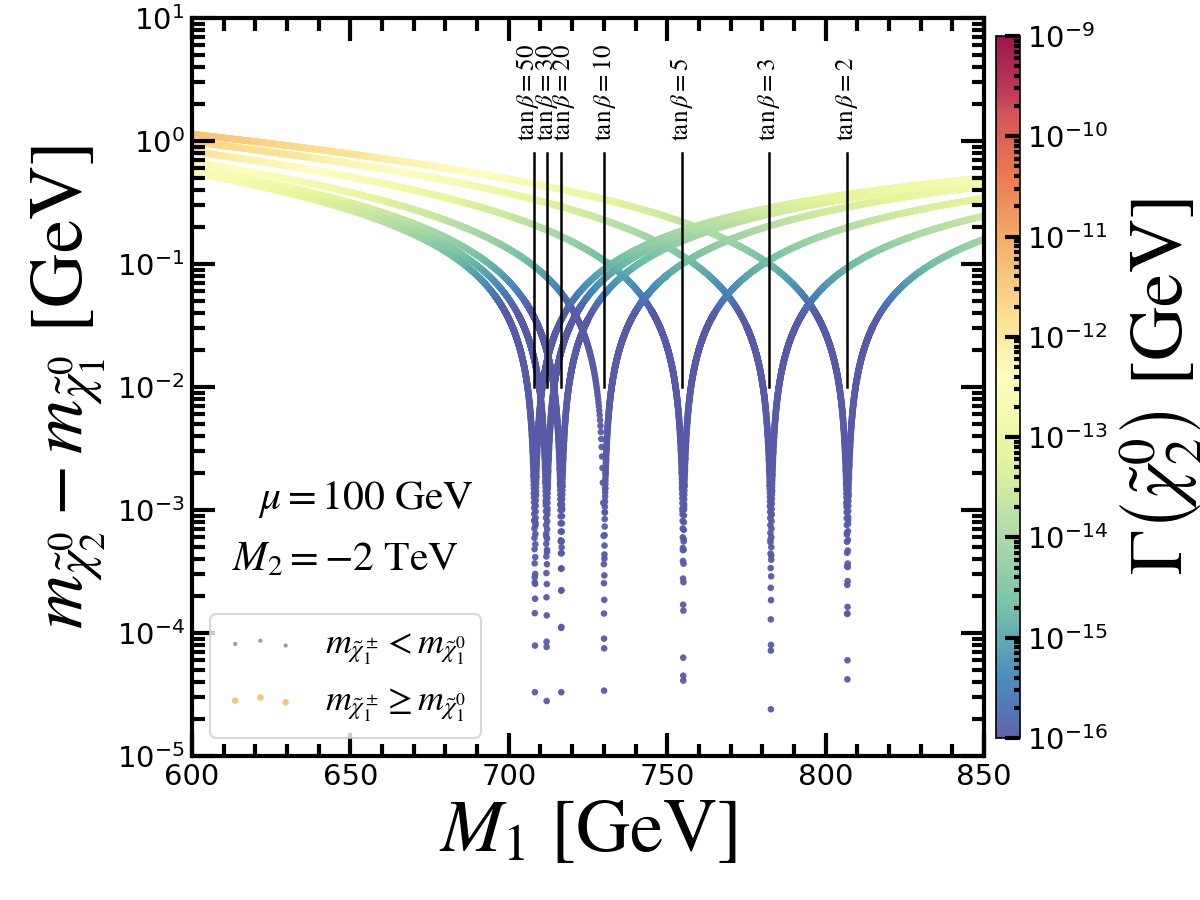
\includegraphics[width=0.495\linewidth]{mu100m.png}
	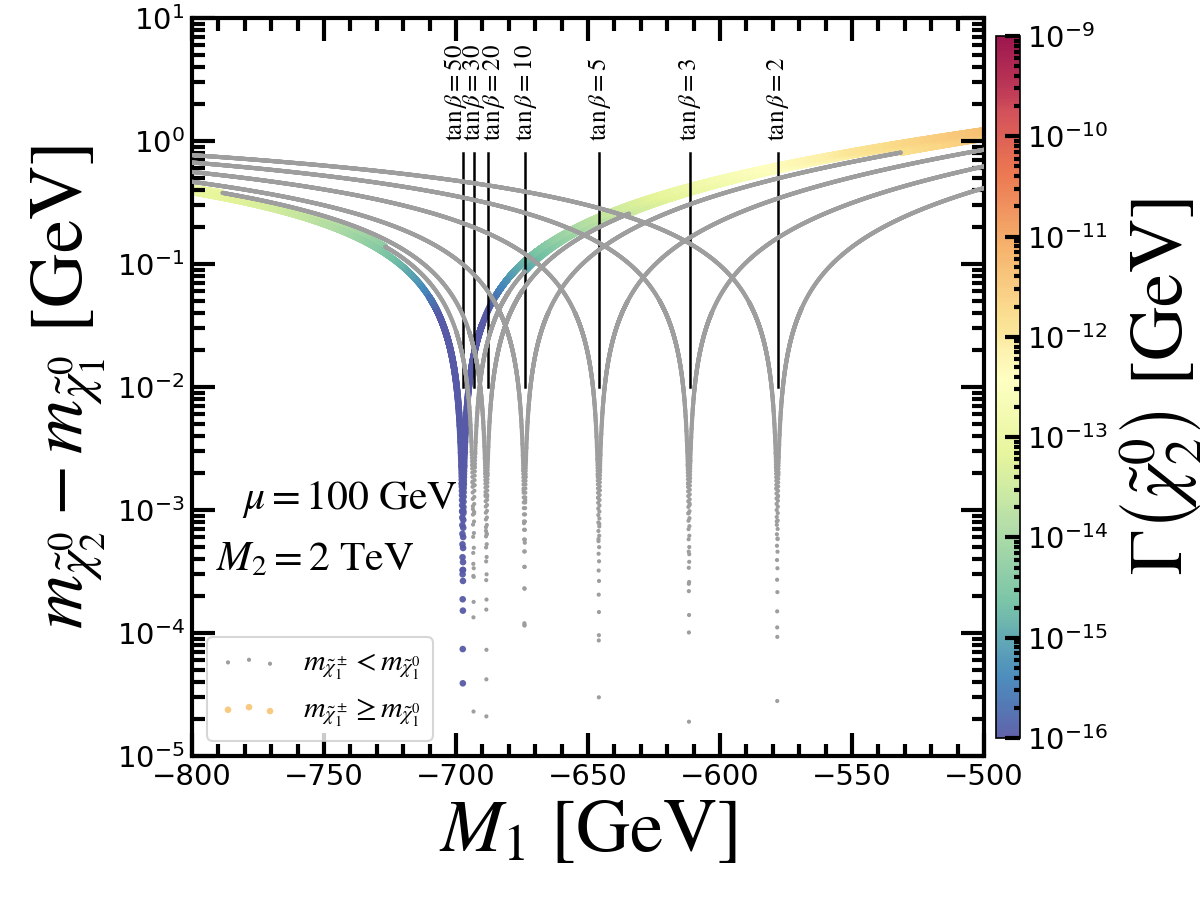
\includegraphics[width=0.495\linewidth]{mu100p.png}

    \vspace{-.3cm}
	\caption{\label{fig:para}The samples projected on the $M_1$ verses $\Delta m^0$ plane, the colour coded with the decay width of the heavier neutrino state $\Gamma_{\tilde{\chi}_2^0}$. The samples coded with grey colour are the charged higgsino $m_{\tilde{\chi}_1^\pm}$ act as the LSP.  }
\end{figure}
\par To further illustrate the cancellation mechanism, we  Figure~\ref{fig:para} illustrates how the mass splitting $\Delta m^0$ between the heavier and lighter neutralino states varies as a function of the gaugino mass parameter $M_1$ for fixed $\mu=100~{\rm GeV}$ and $M_2 = \pm 2~{\rm TeV}$ using the \texttt{SUSYHIT} package.
 As shown in both panels, the mass splitting $\Delta m^0$ exhibits pronounced dips at specific values of $M_1$, corresponding to points where the contributions from $M_1$ and $M_2$ nearly cancel, as described by Eq.~(\ref{eq:msplitn2n1}) and (\ref{eq:sim}). This cancellation leads to an extremely small mass difference and thus a suppressed $\tilde{\chi}_2^0$ decay width $\Gamma(\tilde{\chi}_2^0)$. The colours coding in the figure reflects the decay width, emphasising that near these cancellation points, the heavier higgsino-like neutralino can become very long-lived. The choices of $\tan\beta$  slightly affects the location the maximum cancellation, the ratio of $M_1/M_2$, occurs. Also, when $\mu$ and $M_2$ have the same sign, only the larger value of $\tan{\beta}$ will ensure that chargino $\tilde{\chi}_1^\pm$ is heavier than the lightest neutralino $\tilde{\chi}_2^0$. 
 
In Fig.~\ref{fig:dcmdnm}, we project all samples in Fig.~\ref{fig:para} into $\Delta m^\pm$ verses $\Delta m^0$ panel, with colour coded with $\tan{\beta}$. One can see that, each broken line composed of scattered points contains two line segments with different slopes. This is because $\tilde{H}_1^0$ and $\tilde{H}_2^0$ satisfy the different forms of mass splitting between $\tilde{\chi}_1^\pm$, which is described by Eq.~(\ref{eq:msplitc1H1}) and Eq.~(\ref{eq:msplitc1H2}). When $\tan{\beta}$ tend to be large, the behaviour of $\tilde{H}_1^0$ as the LSP converges to the behavior of $\tilde{H}_2^0$ as the LSP. This is because all beta-related terms in the mass splitting appear in the form of $\sin{2\beta}$. When $\tan{\beta}$ is small, the mass splitting of chargino and LSP is dominated by the term proportional to $(1+\sin{2\beta})$, which is one of the mass corrections from $M_1$ and $M_2$. 
\par Here, we can clearly see that in the general MSSM parameter space of higgsino LSP, the masses of the higgsino triplet approximately satisfy the relation $m_{\tilde{\chi}_1^\pm} \sim \frac{1}{2}(m_{\tilde{\chi}_1^0} + m_{\tilde{\chi}_2^0})$. This arises because the correction terms of $m_Z^2$ in mass splitting $\Delta m^\pm$ and in mass splitting $\Delta m^0$ differ by an overall factor $1/2$. This is the rationale used to simplify the analysis when searching for higgsino. However, in the case of this paper, only chargino $\tilde{\chi}_1^\pm$ can leave hard enough decay products, while neutralino $\tilde{\chi}_1^0$ and $\tilde{\chi}_2^0$ act as missing energy. This makes the exclusion regions drawn in the experiment report do not apply to the situation discussed in this paper.

\begin{figure}[h]
\centering
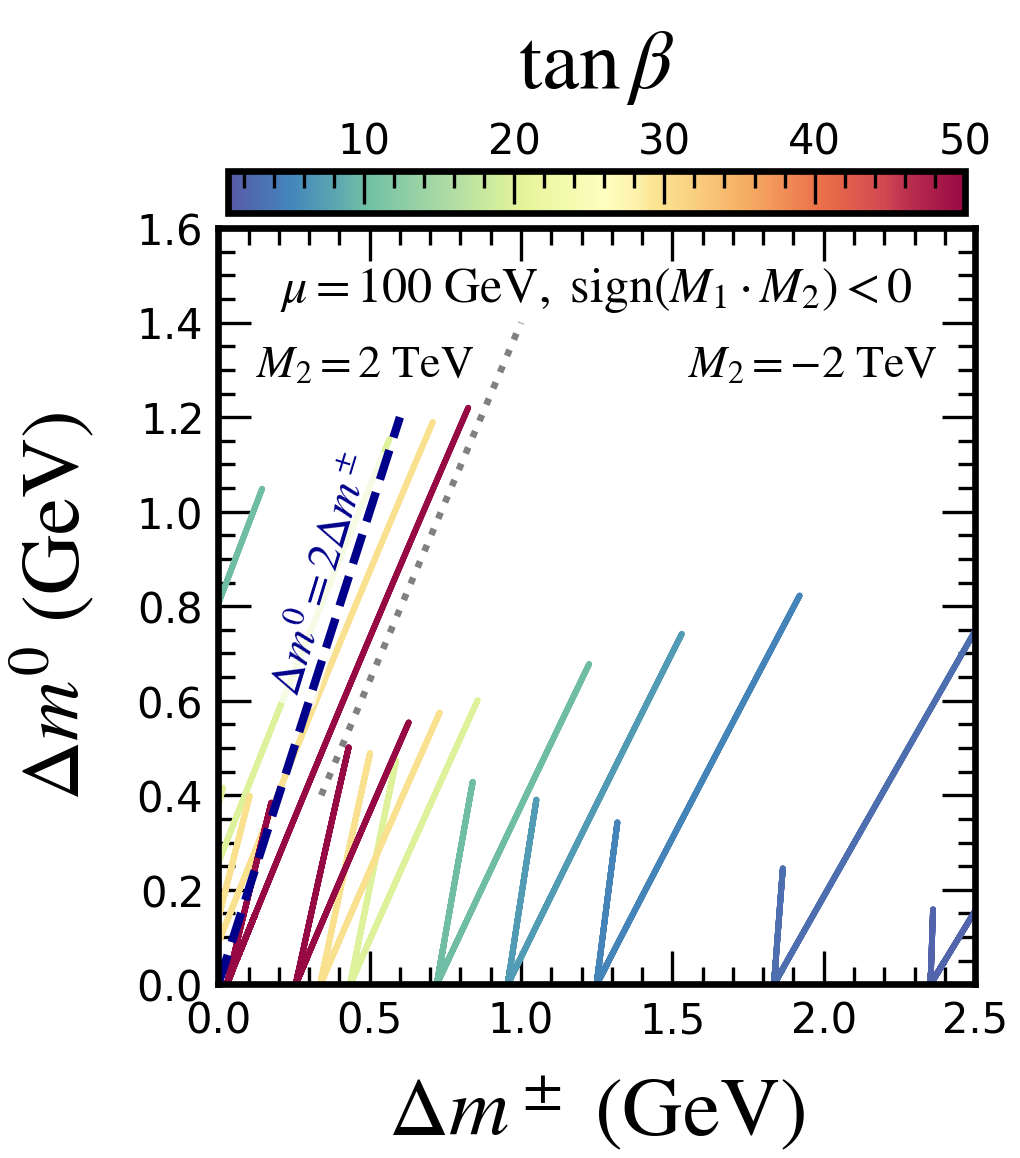
\includegraphics[width=0.6\linewidth]{dmCdmN.png}
\vspace{-.5cm} 
\caption{\label{fig:dcmdnm} Same samples to Fig.~\ref{fig:para}, but in $\Delta m^\pm$ verses $\Delta m^0$ panel.  }
\end{figure}

\par In our case, the mass difference $\Delta m^0$ is very small. Consequently, $\tilde{\chi}_2^0$ primarily decays into $\tilde{\chi}_1^0$ and a $\gamma$, or it undergoes a three-body decay via an off-shell $Z$ boson.
\begin{equation}\begin{split}
	\tilde{\chi}_2^0 &\to \tilde{\chi}_1^0 + \gamma    \\
	&\to \tilde{\chi}_1^0 + Z^* \to \tilde{\chi}_1^0 + f\bar{f}. 
\end{split}\end{equation}
The decay of the neutralino has been thoroughly investigated in Refs.~\cite{Haber:1988px, Gunion:1987yh, Ambrosanio:1995az, Ambrosanio:1996gz, Baer:2002kv}, The numerical calculations are summarized and implemented in the \texttt{SDECAY}~\cite{Djouadi:2006bz}. 
When the mass splitting $\Delta m^0$ is less than 1 GeV, $\tilde{\chi}_2^0$ primarily undergoes radiative decay.
\begin{equation}
	\Gamma(\tilde{\chi}_2^0 \to \tilde{\chi}_1^0 \gamma) = \frac{g_{\tilde{\chi}_2^0 \tilde{\chi}_1^0 \gamma}^2 }{8 \pi } \frac{\left( m_{\tilde{\chi}_2^0}^2 - m_{\tilde{\chi}_1^0}^2 \right)^3}{m_{\tilde{\chi}_2^0}^5},
\end{equation}
where $g_{\tilde{\chi}_2^0 \tilde{\chi}_1^0 \gamma} \propto e g^2 /16\pi^2 $  is an effective coupling arising from the one-loop diagrams.
We have checked that for $\mu$ in the range of $100~{\rm GeV}$ to $500~{\rm GeV}$, the branching ratio of $\tilde{\chi}_2^0$ decays into $\tilde{\chi}_1^0 Z^\star$ is about $30\%$ for a mass splitting of $1~{\rm GeV}$. When the mass splitting reaches below $0.1~{\rm GeV}$, the branching ratio $\text{BR}(\tilde{\chi}_2^0 \to \tilde{\chi}_1^0 Z^\star)$ decreases to less than $1\%$.

\begin{figure}[h]
	\centering
	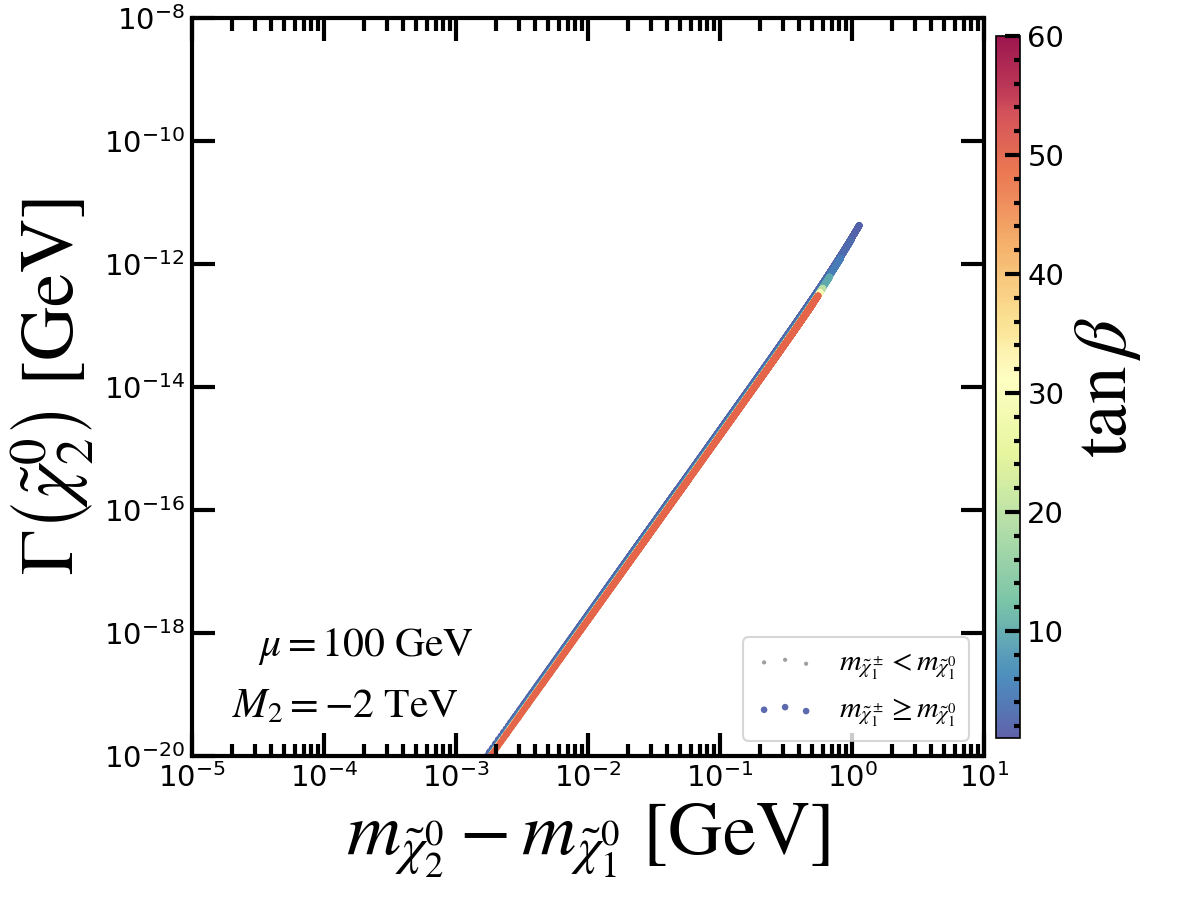
\includegraphics[width=0.495\linewidth]{dkdm100m.png}
	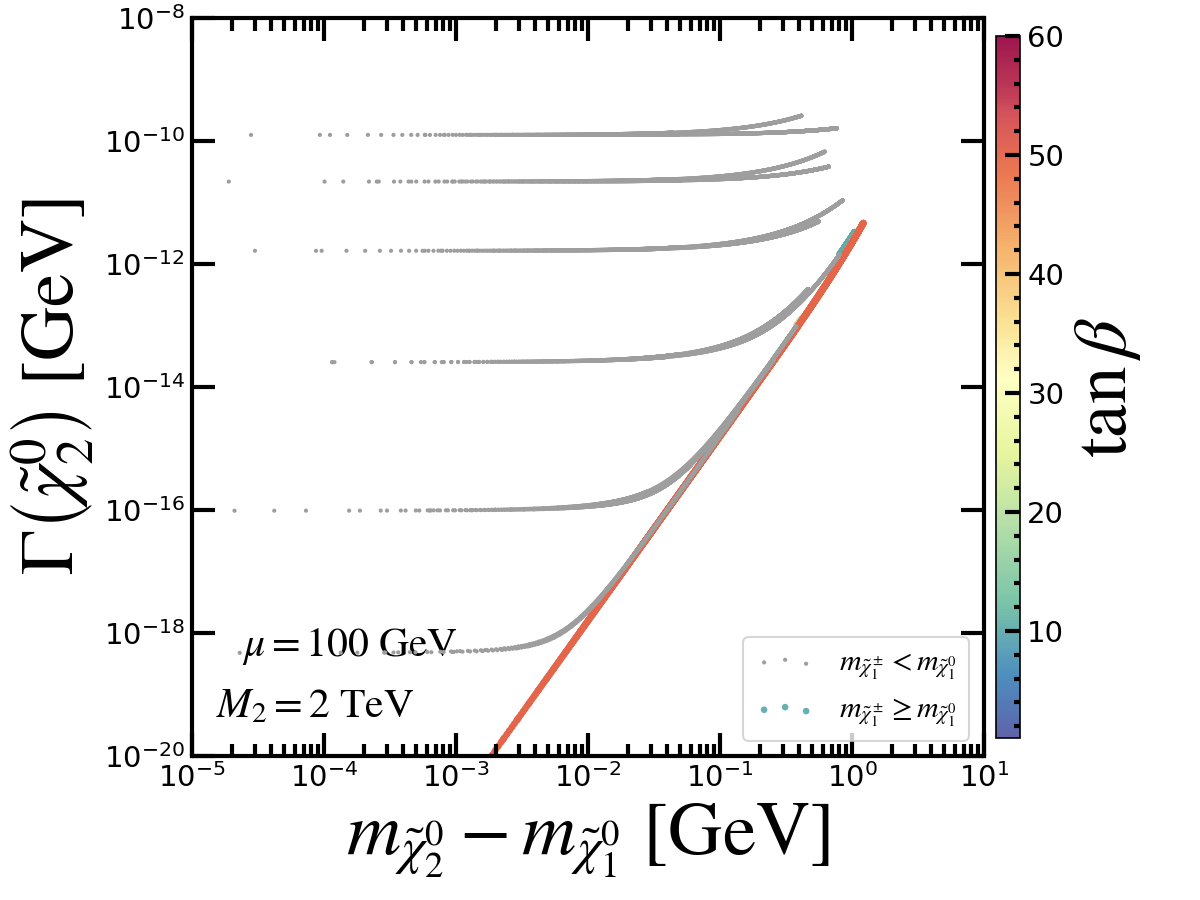
\includegraphics[width=0.495\linewidth]{dkdm100p.png}
    
    \vspace{-.3cm} 
	\caption{\label{fig:dkdm} Same samples to Fig.~\ref{fig:para}, but in $\Gamma(\tilde{\chi}_2^0)$ verses $\Delta m^0$. The color scale indicates the value of $\tan\beta$. The blue dashed lines denote the branching ratio for the decay mode ${\rm BR}(\tilde{\chi}_2^0 \to  \tilde{\chi}_1^0 Z^*)$.  }
\end{figure}
 

Figure~\ref{fig:dkdm} presents the correlation between the decay width of the heavier neutralino, $\Gamma\left(\tilde{\chi}_2^0\right)$, and the mass splitting $\Delta m^0$, using the same samples set as in Fig.~\ref{fig:para}. As seen in the plot, there is an obvious power-law relationship between the decay width and the mass splitting. The effect of $\tan\beta$ on this power law relationship is negligible. 

%%%%%%%%%%%%%% section Model %%%%%%%%%%%%%%%%%
\section{Experimental Constraints}
\label{sec:exp}
%%%%%%%%%%%%%%%%%%%%%%%%%%%%%%%%%%%%%%%%%%%%%%

Current searches for higgsinos at collider experiments, particularly at the LHC, are interpreted by the simplified models in which the higgsino triplet states satisfying specific mass hierarchies and splittings. Therefore, most existing exclusion limits assume that the mass splitting $m_{\tilde\chi_2^0} - m_{\tilde{\chi}_1^0}$ is large enough to generate detectable decay products. In contrast, our scenario features a highly compressed spectrum, with $\tilde{\chi}_2^0$ and the LSP nearly degenerate, so that only charginos $\tilde{\chi}_1^\pm$ can yield visible signals. As a result, exclusion contours end to overestimate the sensitivity for our scenario. 
\begin{itemize}
\item The LEP search for chargino nearly mass degenerate with the lightest neutralino~\cite{Abdallah:2002aik, DELPHI:1999jsl, ALEPH:2002gap, L3:1999twz, DELPHI:1997tcq}. The LEP experiments have analysed the chargino pair production across its four main experiments: ALEPH, DELPHI, L3, and OPAL. The results are categorised by different decay topologies of chargino: 
	\begin{itemize}
	\item For mass splitting $\Delta m \left( \tilde{\chi}_1^\pm, \tilde{\chi}_1^0 \right) > 3~{\rm GeV}$, chargino will prompt decay into $\tilde{\chi}_1^0$ plus an off-shell $W^{\star}$ boson. Searches for direct $\tilde{\chi}_1^+ \tilde{\chi}_1^-$ production by ALEPH detector~\cite{ALEPH:1999tew, ALEPH:2000qvz} excluded the higgsino-dominated chargino mass reach to $101.1~{\rm GeV}$ for mass splitting $\Delta m \left( \tilde{\chi}_1^\pm, \tilde{\chi}_1^0 \right) = 5~{\rm GeV}$. 
	\item For mass splitting less than about $0.1~{\rm GeV}$, chargino is long-lived  and act as a heavy stable particle in detector. Searches~\cite{ALEPH:1997siq, Antonelli:2001exa, ALEPH:2002ijn} based on a specific energy-loss measurement $(dE/dx)$ by the tracking electronics exclude the higgsino mass below $101~{\rm GeV}$.  
	\item For the middle mass splitting region, chargino pair need an initial state radiation (ISR) photon to boost the decay products to sufficiently large energy to activate the trigger system. Search~\cite{ALEPH:2002gap} target on ISR photon in associate with light visible energy sets a lower limit of $91~{\rm GeV}$ for higgsino-dominated chargino mass.
	\end{itemize}
	There are also some searches target on neutralino, such as Ref.~\cite{DELPHI:2000ijd}, but in the scenario of degenerated higgsino spectrum $m_{\tilde{\chi}_2^0} - m_{\tilde{\chi}_1^0} \lesssim 1~{\rm GeV}$, the detection capabilities to higgsino mass are not stronger than those described above.     

	\item The ATLAS search for electroweak production of electroweakino in final states with two or three soft leptons and missing transverse momentum~\cite{ATLAS:2021moa, ATLAS:2019lng}. These searches target on the simplified model in which neutralino-chargino pair decay to $WZ$ bosons, which $Z$-boson in turn decay to a lepton pair $\ell\ell$ and $W$-boson in turn decay to jets~\cite{ATLAS:2019lng} or to light favour leptons $\ell\nu_\ell$~\cite{ATLAS:2021moa}. Signal regions are defined with significant missing transverse momentum of size $E_{\rm T}^{\rm miss}$, lepton pair invariant mass $m_{\ell\ell}$, stransverse mass $m_{\rm T2}$~\cite{Barr:2003rg, Lester:1999tx} and $R_{\rm ISR}$ variable via Recursive Jigsaw Reconstruction technique~\cite{Jackson:2017gcy}. For the higgsino model with the assumption of $m_{\tilde{\chi}_1^\pm} = \left( m_{\tilde{\chi}_1^0} + m_{\tilde{\chi}_2^0} \right) \big/2$, $\tilde{\chi}_2^0$ masses below $193~{\rm GeV}$ are excluded for mass splitting of $9.3~{\rm GeV}$, and the detectability of mass splittings down to mass splittings of $1.5~{\rm GeV}$ at the LEP chargino bounds $92.4~{\rm GeV}$.
	
    \item The ATLAS search for mass-degenerate higgsinos in final states with low-momentum mildly displaced tracks~\cite{ATLAS:2024umc}. This search is optimized for nearly mass-degenerate higgsinos produced in association with an energetic initial state radiation (ISR) jet and $E_{\rm T}^{\rm miss}$, where the $\tilde{\chi}_1^\pm$ is short-lived and decays a small but measurable distance from the interaction point, resulting in a low-momentum (“mildly displaced”) track with transverse momentum of only a few GeV. The search sensitivity peak locate at $\Delta m \left( \tilde{\chi}_1^\pm, \tilde{\chi}_1^0 \right) = 0.6~{\rm GeV}$ with $\tilde{\chi}_1^\pm$ mass about $170~{\rm GeV}$ for the assumption of $m_{\tilde{\chi}_1^\pm} = \left( m_{\tilde{\chi}_1^0} + m_{\tilde{\chi}_2^0} \right) \big/2$. The mass splitting in the range of $0.3~{\rm GeV} < \Delta m \left( \tilde{\chi}_1^\pm, \tilde{\chi}_1^0 \right) < 0.9~{\rm GeV}$ are excluded for the LEP chargino bounds.  
	
	\item The ATLAS search for Long-lived chargino using a disappearing-track signature~\cite{ATLAS:2022rme}. Signal events passing either $E_{\rm T}^{\rm miss}$ trigger or single-lepton trigger are selected containing a disappearing-track, which is a reconstructed charged particle trajectory that suddenly terminates within the tracking detector. This disappearing-track is consistent with the behaviour of a chargino with a lifetime larger than $0.026~{\rm ns}$ (the mass-splitting smaller than $350~{\rm MeV}$). For higgsino-dominated chargino, the detection lower limit on the mass of chargino with mass splitting $\Delta m \left( \tilde{\chi}_1^\pm, \tilde{\chi}_1^0 \right) = 0.2~{\rm GeV}$ can reach to about $500~{\rm GeV}$.  

	\item The ATLAS search for electroweakino in highly compressed mass spectra~\cite{ATLAS:2024woy}. This search is optimised for electroweakino being produced through vector boson fusion. Signal events containing at least two jets with large gap in pseudo-rapidity, large $E_{\rm T}^{\rm miss}$, and no reconstructed lepton. Boosted decision tree is used to screen for those events that is consistent with the SUSY productions. For wino-like $\tilde{\chi}_1^\pm \tilde{\chi}_2^0$ decays into bino-like LSP model, lower limits of wino mass are established to $120~{\rm GeV}$ with mass splitting $\Delta m \left( \tilde{\chi}_1^\pm/ \tilde{\chi}_2^0, \tilde{\chi}_1^0 \right) = 0.2~{\rm GeV}$. With the help of ATLAS colleagues, we reinterpreted result in higgsino model and found that the higgsino detection capability does not exceed $100~{\rm GeV}$.
    
	\item The ATLAS searches for squarks on jets plus $E_{\rm T}^{\rm miss}$ signature~\cite{ATLAS:2020syg, ATLAS:2021kxv}. In general, mono-jet or multi-jets search from ATLAS and CMS are not sensitive to electroweakino model, but energetic jets can originated from ISR that lead to mono-jet or multi-jets plus large $E_{\rm T}^{\rm miss}$ events. Ref.~\cite{Buanes:2022wgm} recasted the general squark searches in light higgsino model and found that the long standing LEP chargino bounds can be push to $99~{\rm GeV}$ for mass splitting $\Delta m \left( \tilde{\chi}_1^\pm, \tilde{\chi}_1^0 \right) = 0.5~{\rm GeV}$.
    
	\item The CMS search for general SUSY compressed mass spectrum~\cite{CMS-PAS-SUS-23-003}. This report focus on a wide range SUSY compressed models, and the signal regions are defined for different final state with ISR. This search use the RJR algorithm to fully reconstruct the full decay tree of symmetric semi-invisible S-system recoiled by ISR-system. The result presented in the model of higgsino-like $\tilde{\chi}_1^\pm \tilde{\chi}_2^0$ decays into $WZ$ final states with $\Delta m \left( \tilde{\chi}_1^\pm/\tilde{\chi}_2^0, \tilde{\chi}_1^0 \right) > 3~{\rm GeV}$ extend the higgsino mass limit to about $160~{\rm GeV}$. 
	\item The CMS search for electroweakino on two or three soft leptons plus $E_{\rm T}^{\rm miss}$~\cite{CMS:2021edw}. This search targets on the process of electroweakino pair produced and in turn decays into $WZ$ leptonic decay channel plus large $E_{\rm T}^{\rm miss}$. The result is interpreted in simplified model assuming a chargino with mass halfway between the two lightest neutralinos with mass splitting $\Delta m \left( \tilde{\chi}_1^\pm, \tilde{\chi}_1^0 \right) \geq  1.5~{\rm GeV}$. Excluded masses reach up to $205~{\rm GeV}$ for $\Delta m \left( \tilde{\chi}_1^\pm, \tilde{\chi}_1^0 \right)$ of $4~{\rm GeV}$ and $150~{\rm GeV}$ for a highly compressed scenario with $\Delta m \left( \tilde{\chi}_1^\pm, \tilde{\chi}_1^0 \right)$ of $1.5~{\rm GeV}$. 
	\item The CMS search for mono-jet plus $E_{\rm T}^{\rm miss}$~\cite{CMS:2021far}. This search is target to events with energetic jets and large missing transverse momentum. Ref.~\cite{Agin:2023yoq} recasted the results and using the higgsino simplified model reinterpreted in $m_{\tilde{\chi}_2^0}$ - $\Delta m(\tilde{\chi}_2^0, \tilde{\chi}_1^0)$ plane via detailed Monte-Carlo simulation. The recasting result show that this CMS mono-jet search can extend the LEP limit of higgsino mass to about $110~{\rm GeV}$ in the assumption of $m_{\tilde{\chi}_1^\pm} = \left( m_{\tilde{\chi}_1^0} + m_{\tilde{\chi}_2^0} \right) \big/2$. 
    \item The CMS search for higgsino with low-momentum isolated tracks~\cite{CMS:2025twk}. This search targets on higgsino DM in final state with one low momentum (soft), isolated track and large missing transverse momentum. A parameterised neutral network was employed to optimise the sensitivity the isolated track from charged higgsino. The decay products of $\tilde{\chi}_2^0$ are not required to be identified in the SR. $\Delta m(\tilde{\chi}_1^\pm, \tilde{\chi}_1^0)$ between $0.28$ and $1.15~{\rm GeV}$ are excluded for a $100~{\rm GeV}$ mass chargino, and $m_{\tilde{\chi}_1^\pm}$ up to 185 GeV are excluded for $\Delta m(\tilde{\chi}_1^\pm, \tilde{\chi}_1^0) = 0.55~{\rm GeV}$. 
    \item The CMS search for compressed electroweakino~\cite{CMS-PAS-EXO-23-017}. This search utilizes the novel soft electron with a transverse momentum ($p_{\rm T}$) reaching up to $1~{\rm GeV}$ to reconstruct the compressed higgsino spectrum in the $WZ$ decay mode. The probing capability for the mass difference $\Delta m(\tilde{\chi}_1^\pm, \tilde{\chi}_1^0)$ extends to $0.5~{\rm GeV}$ for a $100~{\rm GeV}$ higgsino.
    \item The CMS search for a supersymmetry signal of disappearing tracks~\cite{CMS:2023mny}. This search using the ${\rm d}E/{\rm d}x$ energy loss of signal-candidate tracks to probe long-lived SUSY particle. Compared with the ATLAS result~\cite{ATLAS:2022rme}, the search provide a slightly better sensitivity. 

\end{itemize}
\begin{table}[t]
\centering
\renewcommand{\arraystretch}{1.2}
\resizebox{\linewidth}{!}{

\begin{tabular}{l
                ll
                l
                ll
                }
\toprule
\multirow{2}{*}{\textbf{Analysis/Experiment}} 
  & \multicolumn{2}{c}{\textbf{Mass Splitting Sensitivity}} 
  & \multirow{2}{*}{\textbf{Production Mode}} 
  & \multicolumn{2}{c}{\textbf{Decay Mode}} 
 \\
\cmidrule(lr){2-3} \cmidrule(lr){5-6}
  & $\Delta m(\tilde{\chi}_1^\pm,\,\tilde{\chi}_1^0)~[{\rm GeV}]$ 
  & $\Delta m(\tilde{\chi}_2^0,\,\tilde{\chi}_1^0)~[{\rm GeV}]$ 
  & 
  & $\tilde{\chi}_1^\pm$ 
  & $\tilde{\chi}_2^0$ 
 \\
\midrule
LEP2 $\tilde{\chi}_1^\pm$ exclusion~\cite{Abdallah:2002aik, DELPHI:1999jsl, ALEPH:2002gap, L3:1999twz, DELPHI:1997tcq} 
  & $> 0$ & -- 
  & $e^+e^- \to \tilde{\chi}_1^+ \tilde{\chi}_1^- (\gamma)$  
  & $W^{(\star)} \tilde{\chi}_1^0$ 
  & -- 
\\
ATLAS soft-2$\ell$ or 3$\ell$~\cite{ATLAS:2021moa, ATLAS:2019lng}
  & $> 1.5$  & $> 3$ 
  & $\tilde{\chi}_1^\pm \tilde{\chi}_2^0 / \tilde{\chi}_1^0 \tilde{\chi}_2^0 /\tilde{\chi}_1^+ \tilde{\chi}_1^-$ 
  & $W^{(\star)}\tilde{\chi}_1^0 $ 
  & $Z^{(\star)} (\to \ell\ell) \tilde{\chi}_1^0 $ 
\\
CMS soft-2$\ell$ or 3$\ell$~\cite{CMS:2021edw}
  & $1.5 - 10$ & $3 - 20$ 
  & $\tilde{\chi}_1^\pm \tilde{\chi}_2^0 / \tilde{\chi}_1^0 \tilde{\chi}_2^0 $ 
  & $W^{(\star)} (\to \ell \nu)\tilde{\chi}_1^0 $ 
  & $Z^{(\star)} (\to \ell\ell) \tilde{\chi}_1^0 $ 
\\
ATLAS monojet~\cite{ATLAS:2021kxv, Buanes:2022wgm}
& $0.5 - 1.5 $	& $1 - 3$
& $(\tilde{\chi}_1^\pm \tilde{\chi}_2^0  /   \tilde{\chi}_1^\pm \tilde{\chi}_1^0  /  \tilde{\chi}_1^+ \tilde{\chi}_1^-) + {\rm jets}$
& -- & -- 
\\
CMS monojet~\cite{CMS:2021far, Agin:2023yoq}
& $0.45 - 2.5 $	& $0.9 - 5$
& $(\tilde{\chi}_1^\pm \tilde{\chi}_2^0  /   \tilde{\chi}_1^\pm \tilde{\chi}_1^0  /  \tilde{\chi}_1^+ \tilde{\chi}_1^-) + {\rm jets}$
& -- & -- 
\\  
CMS compressed EWino~\cite{CMS-PAS-EXO-23-017}
  & $0.5 - 12 $ & $1 - 25$
  & $\tilde{\chi}_1^\pm \tilde{\chi}_2^0$ + ISR 
  & $W \tilde{\chi}_1^0 $ 
  & $Z \tilde{\chi}_1^0 $ 
\\
ATLAS displaced track~\cite{ATLAS:2024umc}  
  & $0.3 - 0.8$ & --
  & $\tilde{\chi}_1^\pm \tilde{\chi}_{1/2}^0 / \tilde{\chi}_1^+ \tilde{\chi}_1^-$ 
  & a several cm track
  & --  
\\
CMS displaced track~\cite{CMS:2025twk}
& $0.3 - 1.0$ 	& -- 
& $\tilde{\chi}_1^\pm \tilde{\chi}_{1/2}^0 / \tilde{\chi}_1^+ \tilde{\chi}_1^-$
& a several cm track	&	-- 
\\
ATLAS disappearing-track~\cite{ATLAS:2022rme} 
  & $< 0.3$  & --
  & $pp \to \tilde{\chi}_1^\pm \tilde{\chi}_{1/2}^0 / \tilde{\chi}_1^+ \tilde{\chi}_1^- $ + jets 
  & long-lived $\tilde{\chi}_1^\pm$ 
  & -- 
\\
CMS disappearing track~\cite{CMS:2023mny}
 & $< 0.36 $	& -- 
 & $pp \to \tilde{\chi}_1^\pm \tilde{\chi}_{1/2}^0 / \tilde{\chi}_1^+ \tilde{\chi}_1^- $ + jets 
 & long-lived $\tilde{\chi}_1^\pm $	& -- 
  \\
ATLAS EWino di-jet~\cite{ATLAS:2024woy}
  & -- & --  & $\tilde{\chi}_1^\pm \tilde{\chi}_2^0$ + 2 ISR 
  & -- & --
\\
\bottomrule
\end{tabular}
}
\caption{\label{tab:exp} Summary of for higgsino searches at LEP and the LHC. The mass splitting sensitivity ranges correspond to the regions probed by each analysis for a higgsino mass of 100~GeV.
}
\label{tab:higgsino_masssplitting}
\end{table}

% \begin{table}[t]
% \centering
% \resizebox{\columnwidth}{!}{%
% \begin{tabular}{llllclc}
% \toprule
% {\bf Label} 	&& {\bf Production mode} 	&& {\bf Mass model} 	&& $\mathcal{L}$ [${\rm fb}^{-1}$] 	 \\ \toprule 
% LEP2~\cite{Abdallah:2002aik, DELPHI:1999jsl, ALEPH:2002gap, L3:1999twz, DELPHI:1997tcq}	&& $\tilde{\chi}_1^+ \tilde{\chi}_1^- (\gamma) \to W^{+(\star)} W^{-(\star)} \tilde{\chi}_1^0 \tilde{\chi}_1^0 (\gamma)$ && - && - \\ \hline
% %CERN-EP-2021-059
% ATLAS $3\ell$~\cite{ATLAS:2021moa}  		&& $pp \to \tilde{\chi}_1^\pm \tilde{\chi}_2^0 \to W(\to \ell \nu)Z(\to \ell\ell) \tilde{\chi}_1^0 \tilde{\chi}_1^0$ 						&& $m_{\tilde{\chi}_1^\pm} = \left( m_{\tilde{\chi}_1^0} + m_{\tilde{\chi}_2^0} \right) \big/2$ 	&& $139$  \\ \hline
% %CERN-EP-2019-242
% \multirow{2}{*}{ATLAS soft-$2\ell$~\cite{ATLAS:2019lng}} 		&& $pp \to \tilde{\chi}_1^\pm \tilde{\chi}_2^0 ~ / ~ \tilde{\chi}_1^0 \tilde{\chi}_2^0 ~/~ \tilde{\chi}_1^+ \tilde{\chi}_1^- ; $ 	&& \multirow{2}{*}{$m_{\tilde{\chi}_1^\pm} = \left( m_{\tilde{\chi}_1^0} + m_{\tilde{\chi}_2^0} \right) \big/2$} && \multirow{2}{*}{139} \\
% 		&& $\tilde{\chi}_1^\pm \to  W(\to jj)\tilde{\chi}_1^0,\quad \tilde{\chi}_2^0 \to Z(\to \ell\ell) \tilde{\chi}_1^0$ && &&  \\ \hline
% %CERN-EP-2024-012
% \multirow{3}{*}{ATLAS displaced-track~\cite{ATLAS:2024umc}}		&& $pp\to \tilde{\chi}_1^\pm \tilde{\chi}_2^0 ~ / ~ \tilde{\chi}_1^0 \tilde{\chi}_2^0 ~/~ \tilde{\chi}_1^+ \tilde{\chi}_1^- ~/~ \tilde{\chi}_1^\pm \tilde{\chi}_1^0 $; && \multirow{3}{*}{$m_{\tilde{\chi}_1^\pm} = \left( m_{\tilde{\chi}_1^0} + m_{\tilde{\chi}_2^0} \right) \big/2$}	&& \multirow{3}{*}{140}	 \\
% 	&& $\tilde{\chi}_1^{\pm} \to \pi^\pm \tilde{\chi}_1^0 ~/~ \ell \nu \tilde{\chi}_1^0 $ && &&  \\
% 	&& $\tilde{\chi}_2^{0} \to \pi^+ \pi^- \tilde{\chi}_1^0 ~/~ \ell \ell \tilde{\chi}_1^0 ~/~\pi^0 \tilde{\chi}_1^0 $ && && \\ \hline 
% %CERN-EP-2021-209
% \multirow{2}{*}{ATLAS disappearing-track~\cite{ATLAS:2022rme}} 		&& $pp \to (\tilde{\chi}_1^\pm \tilde{\chi}_2^0 ~ / ~ \tilde{\chi}_1^\pm \tilde{\chi}_1^0 ~/~ \tilde{\chi}_1^+ \tilde{\chi}_1^-) + {\rm ISR}; $ 	&& \multirow{2}{*}{-} && \multirow{2}{*}{136} 				\\
% 		&& $\tilde{\chi}_1^\pm \to \pi^+ \tilde{\chi}_1^0$ (disappearing-track)				&& && \\ \hline	
% %CERN-EP-2024-246
% ATLAS VBF di-jets~\cite{ATLAS:2024woy} 		&& $pp \to (\tilde{\chi}_1^\pm \tilde{\chi}_2^0 ~ / ~ \tilde{\chi}_1^\pm \tilde{\chi}_1^0 ~/~ \tilde{\chi}_1^+ \tilde{\chi}_1^-) + jj; $ 	&& $m_{\tilde{\chi}_1^\pm} = m_{\tilde{\chi}_2^0}$ && 136 				\\ \hline	
% %CERN-EP-2020-166 
% ATLAS mono-jet~\cite{ATLAS:2021kxv, Buanes:2022wgm}		&& \multirow{2}{*}{$pp \to (\tilde{\chi}_1^\pm \tilde{\chi}_2^0 ~ / ~ \tilde{\chi}_1^\pm \tilde{\chi}_1^0 ~/~ \tilde{\chi}_1^+ \tilde{\chi}_1^-) + {\rm jets} $} && \multirow{2}{*}{-} && 139 \\
% %CERN-EP-2020-238
% ATLAS multi-jets~\cite{ATLAS:2020syg, Buanes:2022wgm}		&& && && 139 \\ \hline
% %CMS-PAS-SUS-23-003
% CMS compressed (RJR)~\cite{CMS-PAS-SUS-23-003}		&& $pp \to \tilde{\chi}_1^\pm \tilde{\chi}_2^0 \to WZ \tilde{\chi}_1^0 \tilde{\chi}_1^0$ && $m_{\tilde{\chi}_1^\pm} = m_{\tilde{\chi}_2^0}$ && 138	\\ \hline
% %CMS-SUS-18-004
% \multirow{2}{*}{CMS soft $2/3\ell$~\cite{CMS:2021edw}}		&& $pp \to \tilde{\chi}_1^\pm \tilde{\chi}_2^0 ~/~ \tilde{\chi}_2^0 \tilde{\chi}_1^0 $  && \multirow{2}{*}{$m_{\tilde{\chi}_1^\pm} = \left( m_{\tilde{\chi}_1^0} + m_{\tilde{\chi}_2^0} \right) \big/2$}  && \multirow{2}{*}{137} 	 \\
% 	&& $\tilde{\chi}_1^\pm \to W (\to \ell \nu) \tilde{\chi}_1^0, \quad \tilde{\chi}_2^0 \to Z(\to \ell \ell) \tilde{\chi}_1^0 $ && && \\ \hline
% %CMS-EXO-20-004
% CMS mono-jet~\cite{CMS:2021far, Agin:2023yoq} && $pp \to \tilde{\chi}_1^0 \tilde{\chi}_2^0 ~/~ \tilde{\chi}_1^\pm \tilde{\chi}_2^0 ~/~ \tilde{\chi}_1^\pm \tilde{\chi}_1^0 ~/~ \tilde{\chi}_1^+ \tilde{\chi}_1^-$ 	&& $m_{\tilde{\chi}_1^\pm} = \left( m_{\tilde{\chi}_1^0} + m_{\tilde{\chi}_2^0} \right) \big/2$ 	&& 101  \\ \hline
% %CMS-PAS-SUS-24-012
% CMS isolated track~\cite{CMS:2025twk}	&&	$pp \to \tilde{\chi}_1^\pm \tilde{\chi}_2^0 ~/~ \tilde{\chi}_1^\pm \tilde{\chi}_1^0 ~/~ \tilde{\chi}_1^+ \tilde{\chi}_1^-$	&& - && 138  \\
% \toprule
% \end{tabular}}
% \caption{\label{tab:exp} Summary of representative collider searches for higgsinos at LEP and the LHC. \px{The labels are a bit unclear and need to be updated}}
% \end{table}

\begin{figure}[ht]
	\centering
	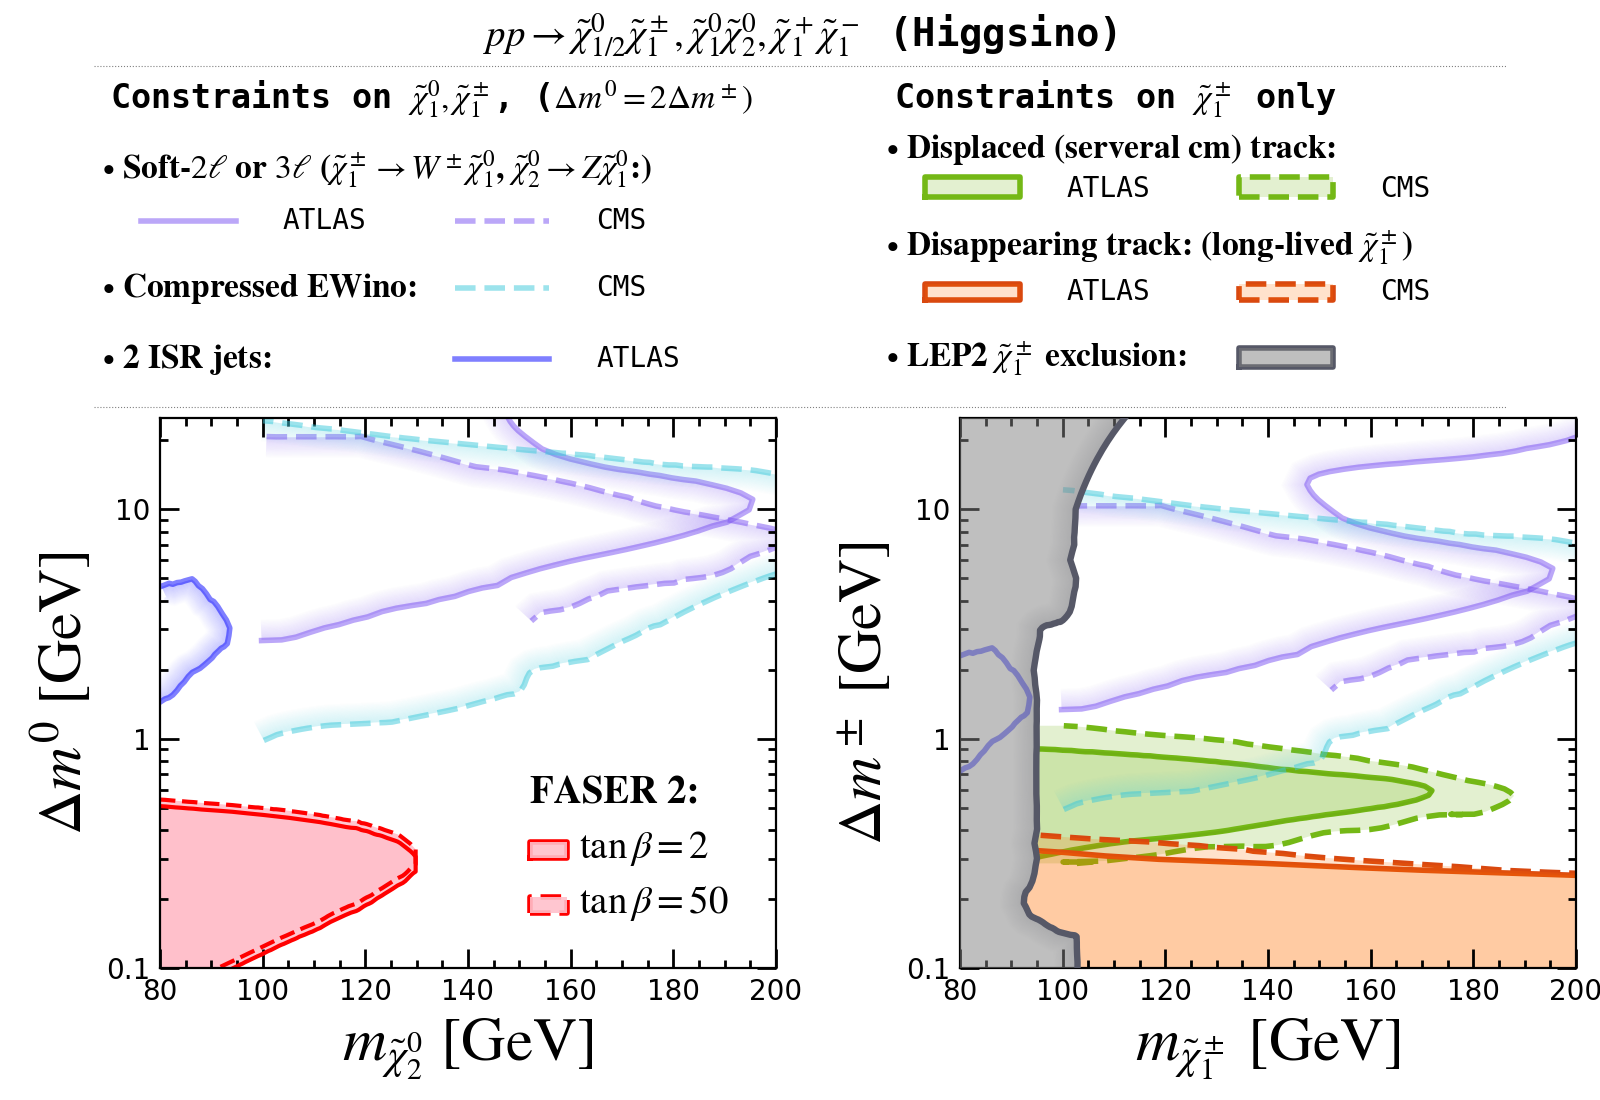
\includegraphics[width=\linewidth]{exp_constrain.png}
    
    \vspace{-.5cm}
	\caption{\label{fig:expconstrain} Exclusion regions of compressed higgsino scenario in the plane of $m_{\tilde{\chi}_2^0}$ versus $\Delta m^0$ (left), and in the plane of $m_{\tilde{\chi}_1^\pm}$ versus $\Delta m^\pm$ (right). The shaded regions indicate various LHC searches from ATLAS and CMS, such as soft-leptons, mono-jet, displaced track, disappearing track, and electroweakino searches. The grey shaded area represents the LEP2 exclusion. The red shaded region represents the projected sensitivity of the FASER 2 experiment.}
\end{figure}

For the sake of intuition, we summaries the $95\%$ confidence level exclusion contour of the directly searches by the above colliders reports based on simplified models in Fig.~\ref	{fig:expconstrain}, and the corresponding simplified model are summarized in Table.~\ref{tab:exp}, focusing on the mass splitting intervals explored for a higgsino mass of 100~GeV. For the scenarios considered in this work, two mass splittings  $\Delta m(\tilde{\chi}_1^\pm,\,\tilde{\chi}_1^0)$ 
  and $\Delta m(\tilde{\chi}_2^0,\,\tilde{\chi}_1^0)$ are not strongly correlated and should be treated as independent parameters.
In particular, for the case of a long-lived neutralino, it can be seen from Table~\ref{tab:exp} and Fig.~\ref{fig:expconstrain} that probing this scenario at the LHC requires the $\Delta m(\tilde{\chi}_1^\pm,\,\tilde{\chi}_1^0)$ mass splitting to be larger than approximately $1~{\rm GeV}$.


%%%%%%%%%%%%%%%%%% Section FASER %%%%%%%%%%%%%%%
\section{FASER sensitivity to long-lived higgsino}
\label{sec:faser}
%%%%%%%%%%%%%%%%%% Overview %%%%%%%%%%%%%%%%%%%%
\subsection{Overview of the FASER Experiment}
The FASER~\cite{Feng:2022inv, FASER:2018eoc} is installed in a service tunnel at a distance
\begin{equation*}
	L = 480~\rm{m}
\end{equation*}
downstream of the ATLAS interaction point (IP), precisely on the beam collision axis. At this location the proton beams have been bent clear by LHC magnets, while neutral LLPs continue in straight trajectories into the detector.  The detector is a compact cylindrical aligned with the beam axis. Key detector parameters for FASER and its proposed FASER 2 upgrade can be summarised as:
\begin{equation}\begin{split}
	&\text{FASER}: \quad 
	R = 0.1~{\rm m}, \quad
	D = 1.5~{\rm m},\quad
	\mathcal{L}_{\rm int} = 150~{\rm fb}^{-1};  \\
	&\text{FASER 2}: \quad 
	R = 1~{\rm m}, \quad 
	D = 5.0~{\rm m}, \quad
	\mathcal{L}_{\rm int} = 3~{\rm ab}^{-1},
\end{split}\end{equation}
where $R$ and $D$ are the radius and length of the detector cylinder.   
\par FASER and FASER 2 are designed to efficiently reconstruct LLPs whose decay products—such as electrons, muons, photons, and hadrons—are highly collimated along the beam direction. To enhance sensitivity to photon final states, a preshower detector based on monolithic silicon pixel sensors has been proposed~\cite{Boyd:2803084}. This enables the efficient detection of photons resulting from $\tilde{\chi}_2^0$ decays.

\par For a LLP with mass $m$ produced at the IP with momentum $p$, angle $\theta$ with respect to the beam axis and the decay width $\Gamma$, the probability that it will decay within the detector volume of FASER is
\begin{equation}\label{eq:Faserprob}
\begin{split}
		{\rm Prob}({\rm FASER}) &= e^{-\frac{(L+D) m \Gamma}{p}} \left( e^{\frac{D m\Gamma}{p}} -1\right) \Theta(R-\tan{\theta}L), \\
		&\approx \frac{D}{\lambda} e^{-\frac{L}{\lambda}} \Theta(R-\tan{\theta}L). 
\end{split} 
\end{equation}
Here, $\Theta(x)$ denotes the Heaviside step function, and the characteristic decay length $\lambda$ of the LLP in the laboratory frame is
\begin{equation}
	\lambda = c \tau \beta \gamma  = \frac{p}{m\Gamma},
\end{equation}
where $\tau=1/\Gamma$ is the proper lifetime (with total width $\Gamma$), and $\beta=v/c$ and $\gamma=1/\sqrt{1-\beta^2}$ are the usual Lorentz factors.

% \subsection{Overview of MATHUSLA Experiment}
% MATHUSLA is a proposed surface detector designed to search for long-lived particles (LLPs) produced at the CMS IP. It is situated approximately 100 meters above the LHC, covering a box-shaped detector volume. Three benchmark design are featured by the fiducial decay volumes: 
% \begin{equation}\begin{split}
% 	{\rm MATHUSLA40}:~ 
% 	&82~{\rm m} \leq x \leq 93~{\rm m},\quad
% 	-20~{\rm m} \leq y \leq 20~{\rm m},\quad
% 	70~{\rm m} \leq z \leq 110~{\rm m};  \\
% 	{\rm MATHUSLA100}:~ 
% 	&60~{\rm m} \leq x \leq 85~{\rm m},\quad
% 	-50~{\rm m} \leq y \leq 50~{\rm m},\quad 
% 	68~{\rm m} \leq  z \leq 168~{\rm m};  	\\
% 	{\rm MATHUSLA200}:~ 
% 	&100~{\rm m} \leq x \leq 120~{\rm m},\quad 
% 	-100~{\rm m} \leq y \leq 100~{\rm m},\quad 
% 	100~{\rm m} \leq  z \leq 300~{\rm m};  	
% \end{split}\end{equation}
% optimized for reconstructing charged particle tracks from LLP decays in a low-background environment \cite{MATHUSLA:2025eth, MATHUSLA:2025zyt}.

% \px{I see that the MATHUSLA will not provide any sensitiviy to the scenario of higgsino-like $\tilde{\chi}_2^0$, if MATHUSLA can not reconstruct the photons }

\subsection{Expected sensitivity to Long-lived higgsino}

\px{The differential cross section of chi production is enhanced at $\theta \to 0$. How to show this property? via formula or differential distribution of $\theta$?}

 

\begin{figure}
    \centering
    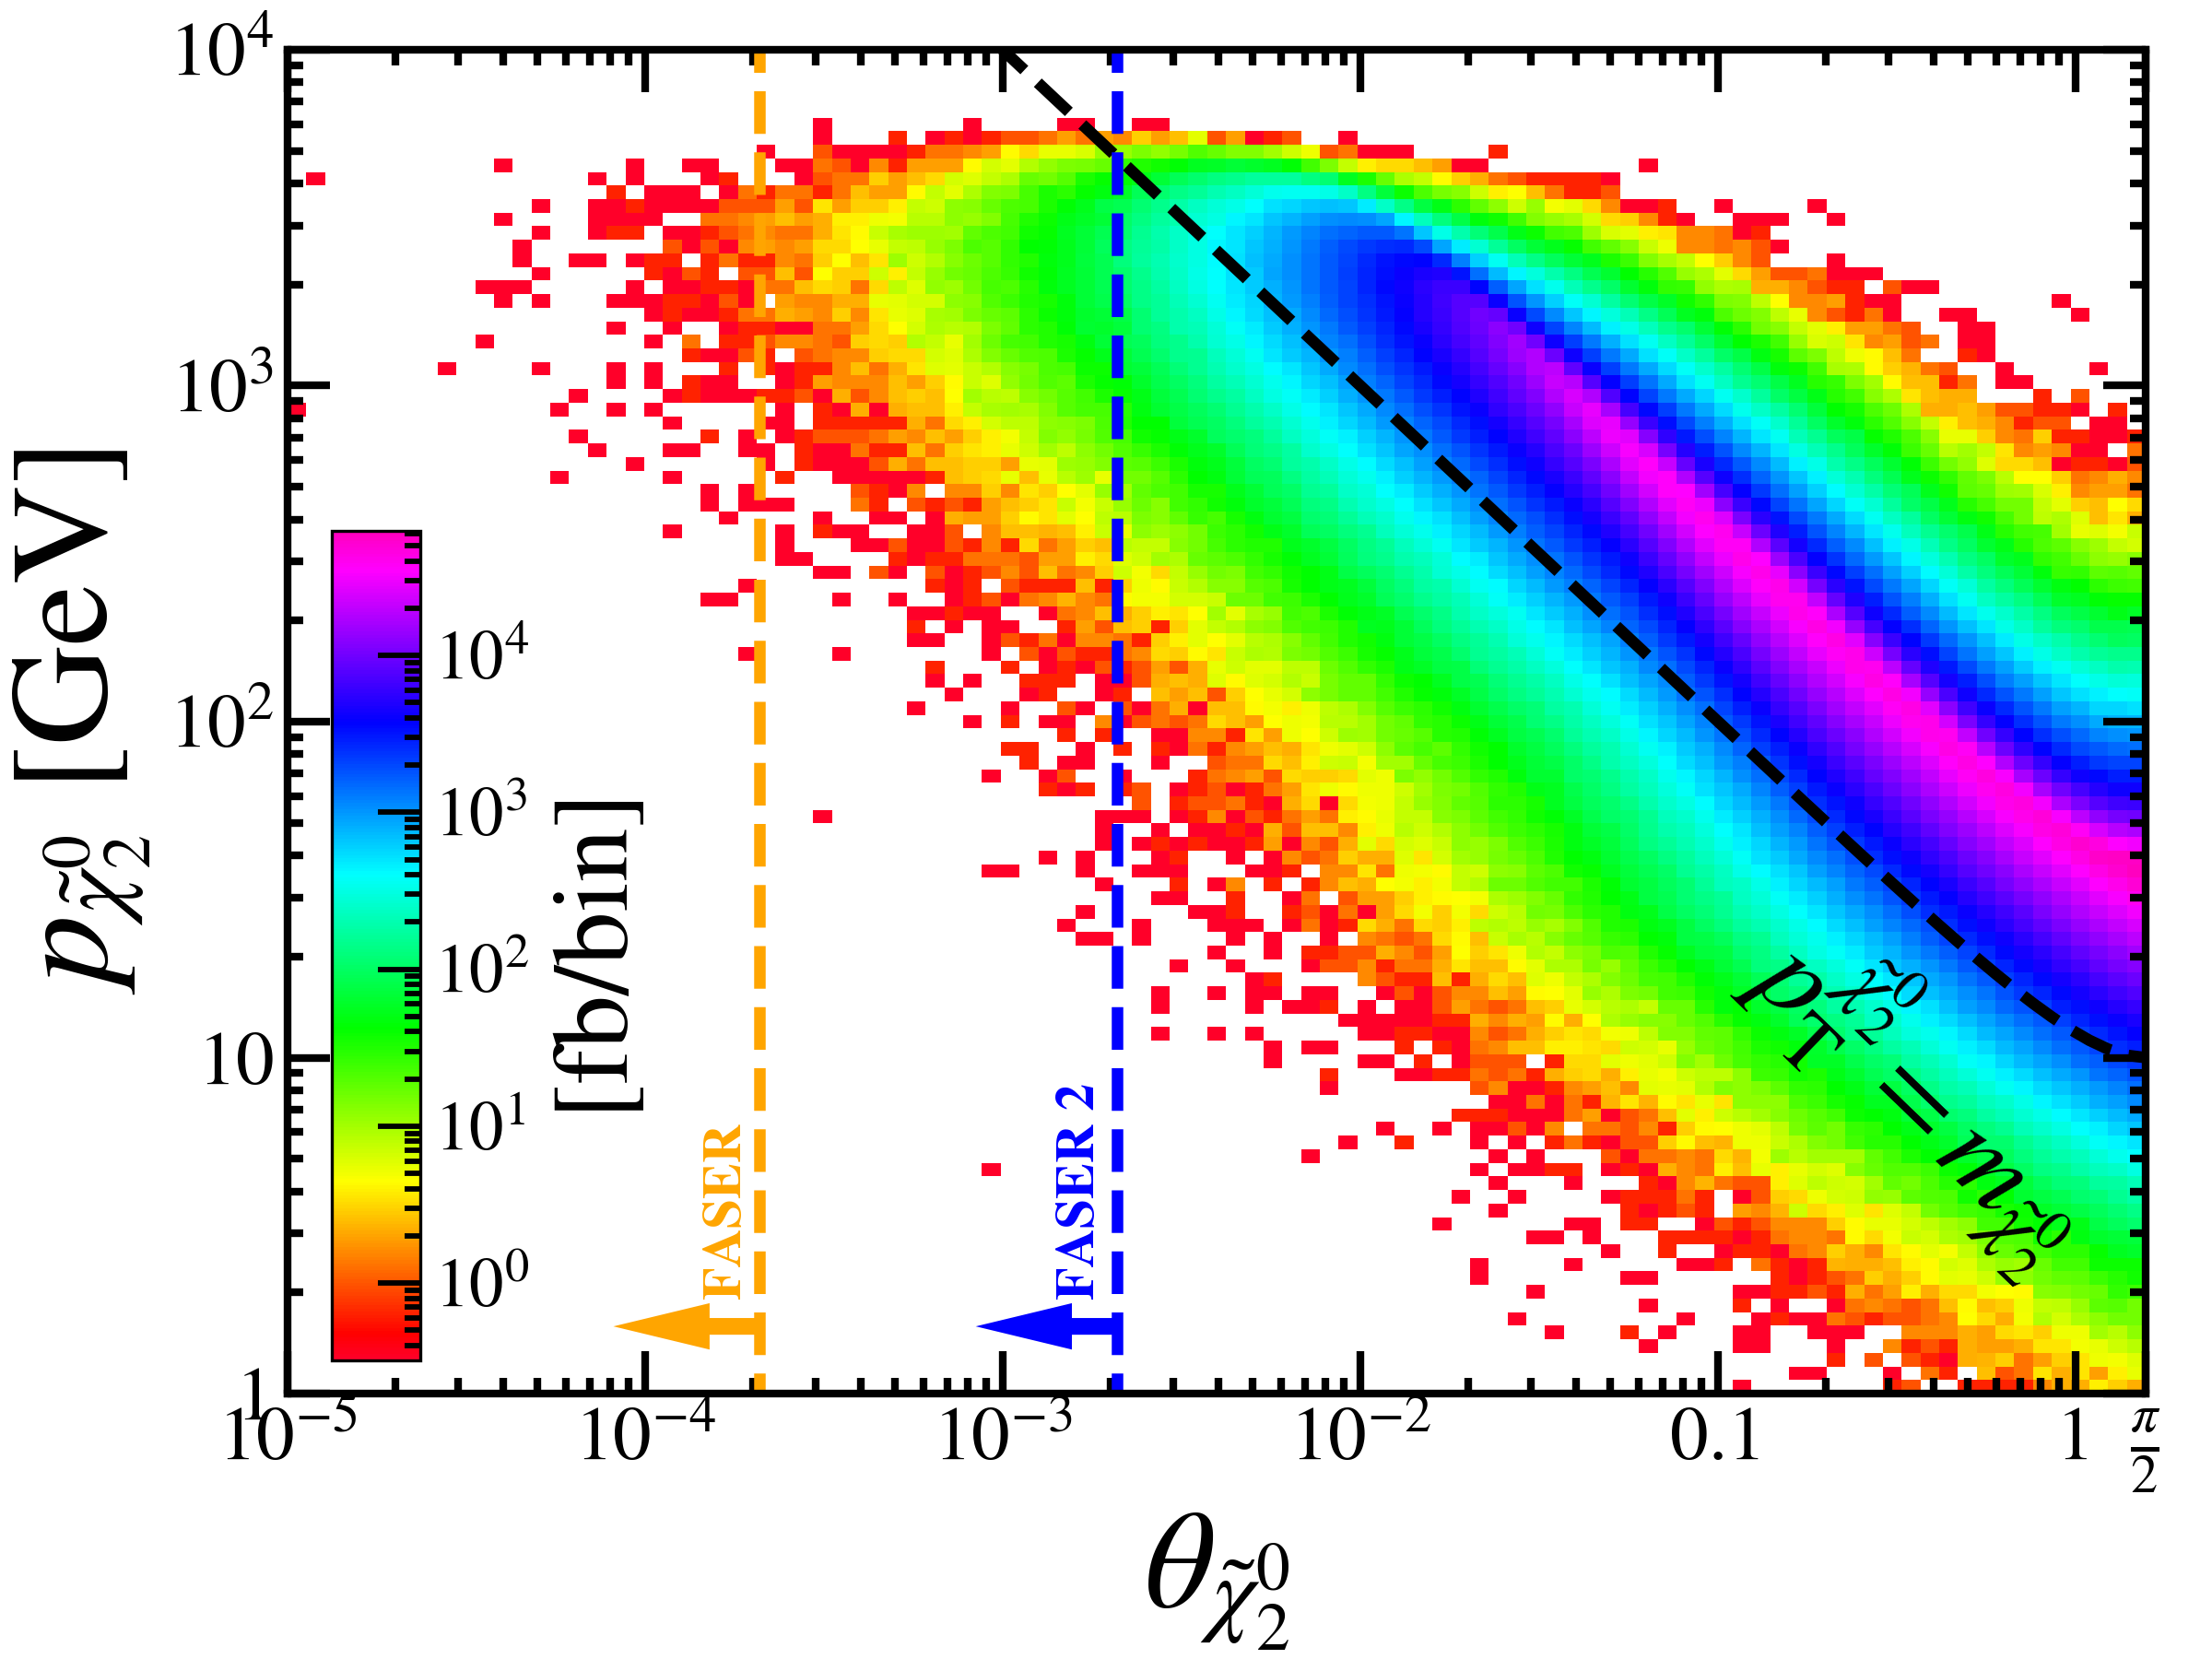
\includegraphics[width=0.495\linewidth]{10-distri.png}
    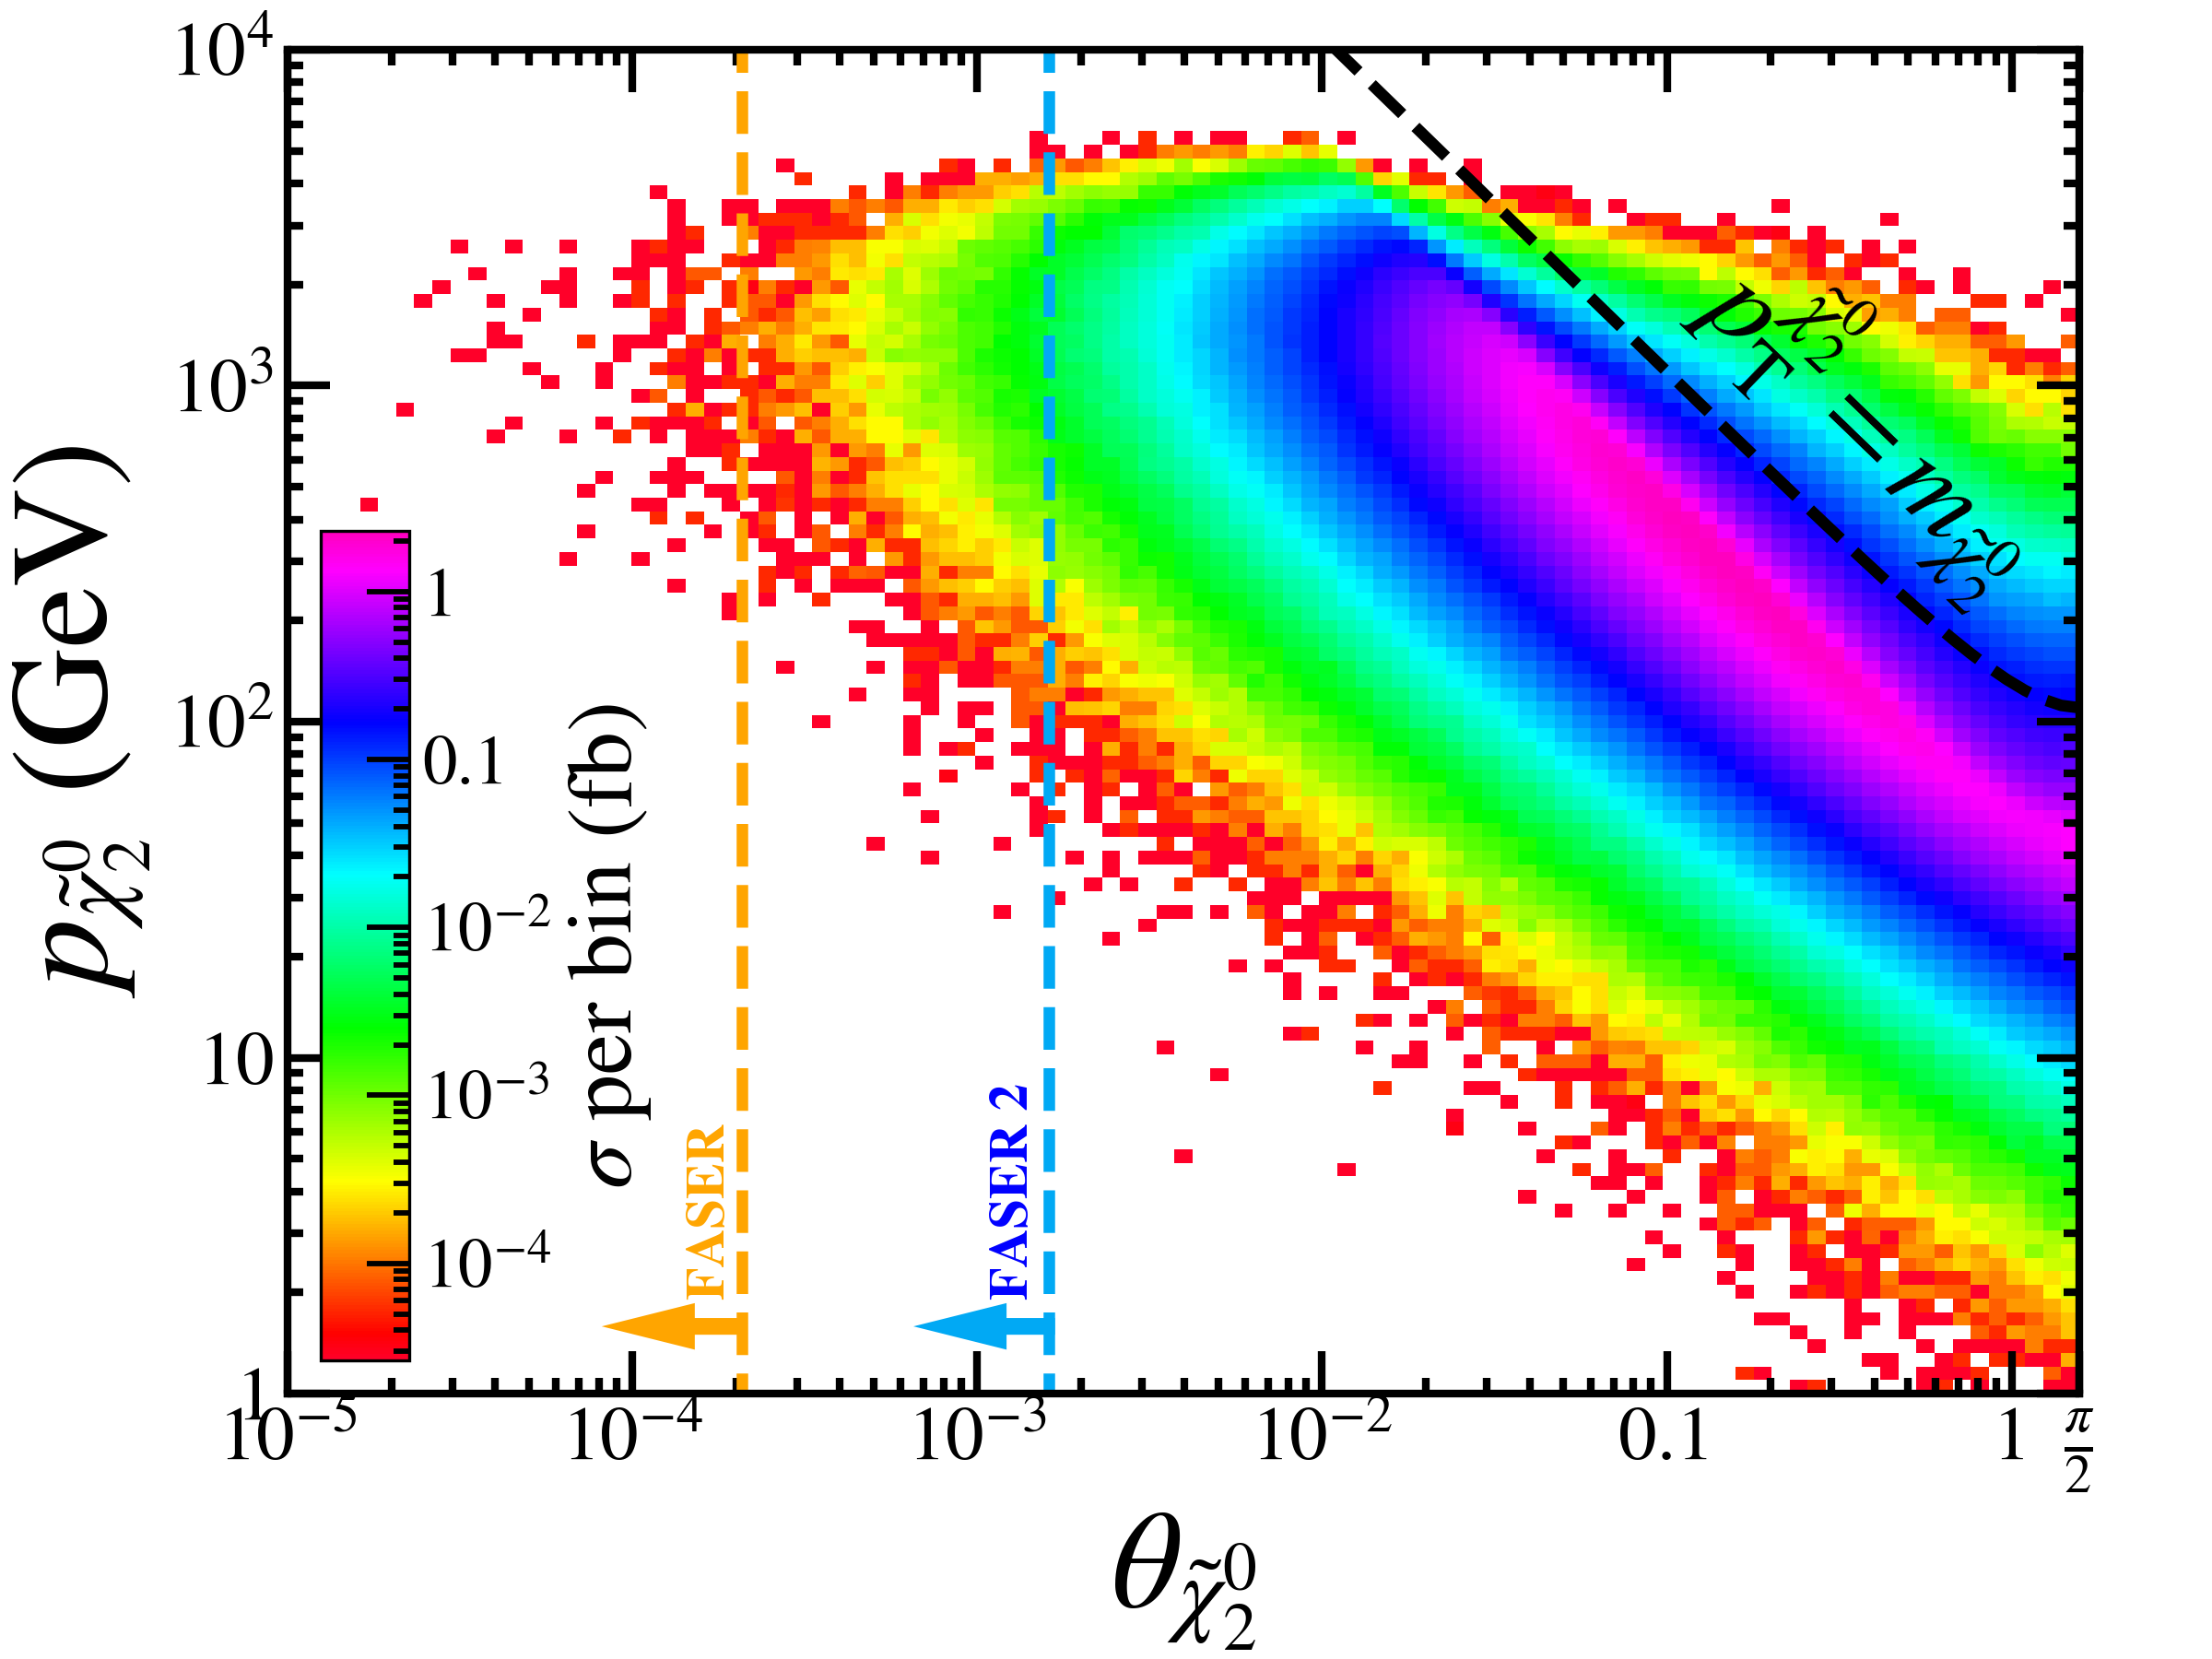
\includegraphics[width=0.495\linewidth]{110-distri.png}

    \vspace{-.3cm}
\caption{\label{fig:xsect} Density map of the heavier neutralinos lab-frame momentum $p_{\tilde\chi^0_2}$ versus its polar angle $\theta_{\tilde\chi^0_2}$ for $\tilde\chi^0_2\tilde\chi^\pm$ production at LHC, shown for higgsino mass parameter $\mu = 10~{\rm GeV}$ (left) and $\mu = 110~{\rm GeV}$ (right).  The logarithmic color scale shows the cross section per bin in unit of ${\rm fb}$. The vertical dashed lines (with arrows) indicate the angular acceptances of FASER (orange) and FASER 2 (blue).  The black dashed curve follows the kinematic relation $p^{\tilde{\chi}_2^0}_{\rm T} = m_{\tilde{\chi}_2^0}$.}
\end{figure}

Different from the benchmark scenario in Ref.~\cite{FASER:2018eoc}, the special feature of the compressed higgsino scenario in this work is that it is an electroweak hard process. When other supersymmetric particles are decoupled, higgsino pairs are mainly produced at the LHC via a $s$-channel $Z$ boson or $W$ boson~\cite{Haber:1984rc}. 
\par To perform a numerical result, we use the Monte-Carlo event generator \texttt{Pythia83}~\cite{Bierlich:2022pfr} with the Monash tune~\cite{Skands:2014pea} to generate the production of $\tilde{\chi}_1^0 \tilde{\chi}_2^0$, $\tilde{\chi}_i^0 \tilde{\chi}_1^\pm$ at LHC. Then for each event, select the $\tilde{\chi}_2^0$ candidate and use Eq.~(\ref{eq:Faserprob}) to calculate the probability of its decay in FASER or FASER 2 detector. 
As shown in Fig.~\ref{fig:xsect}, the production rates of $\tilde{\chi}_2^0$ with $\mu$ of $10~{\rm GeV}$ and $100~{\rm GeV}$ are projected in the $(\theta, p)$ planes, where $\theta$ and $p$ are the higgsino-like neutralino $\tilde{\chi}_2^0$'s angle with respect to the beam axis and momentum, respectively. The momentum of $\tilde{\chi}_2^0$ is negatively correlated with its angle respect to the beam axis. Relatively, the production rate of $\tilde{\chi}_2^0$ increase at small $\theta$, but decrease rapidly in region of $\theta \lesssim 0.01$. This results in an insufficient event of $\tilde{\chi}_2^0$ in FASER, but a sufficient generation rate in FASER 2. Inside the FASER 2 region, the momentum carried by $\tilde{\chi}_2^0$ is mainly ranges from about 500 GeV to several TeV, indicating that $\tilde{\chi}_2^0$ is highly boosted. 
%Therefore, for the case of smaller mass splitting at about $0.1~{\rm GeV}$, the visible decay products of the long-lived higgsino state $\tilde{\chi}_2^0$ are hard enough to trigger signal events in the detector. 
\px{What is the visible energy threshold of FASER 2? Evis $>$ 100 GeV? if so, the FASER 2 sensitivity of Long-lived higgsino will not expected to reach over 100 GeV. due to the Evis $\sim \Delta m * p(N2)/m(N2) $. For a 100 GeV N2, p=3 TeV, mass splitting of 0.1 GeV, the visible energy will only 3 GeV. }

\begin{equation}
    \mu(\rho) = \frac{1}{3} \sum_{i,j \in k,n,r} C_{ij}^2
\end{equation}

\begin{figure} 
\centering
    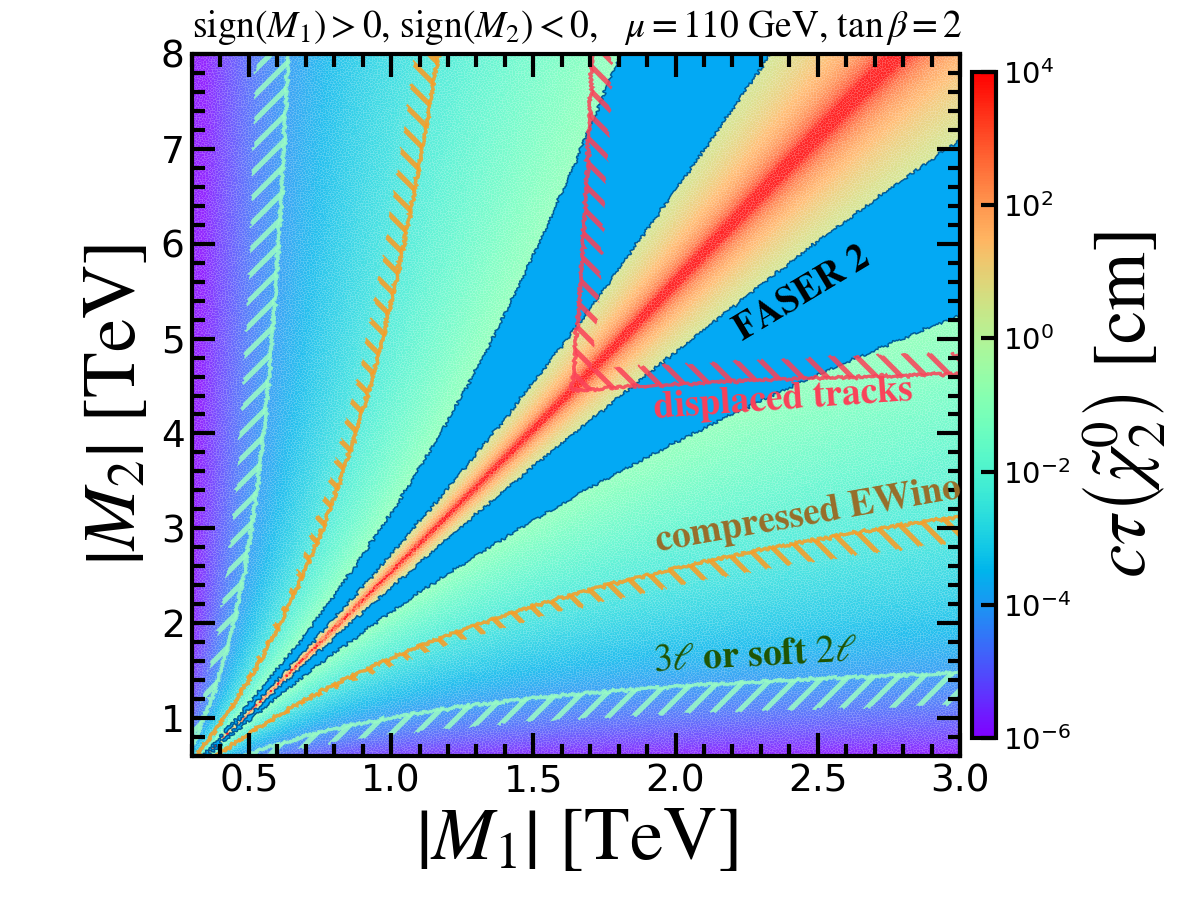
\includegraphics[width=0.495\linewidth]{mu110_TB02_M2minus.png}
    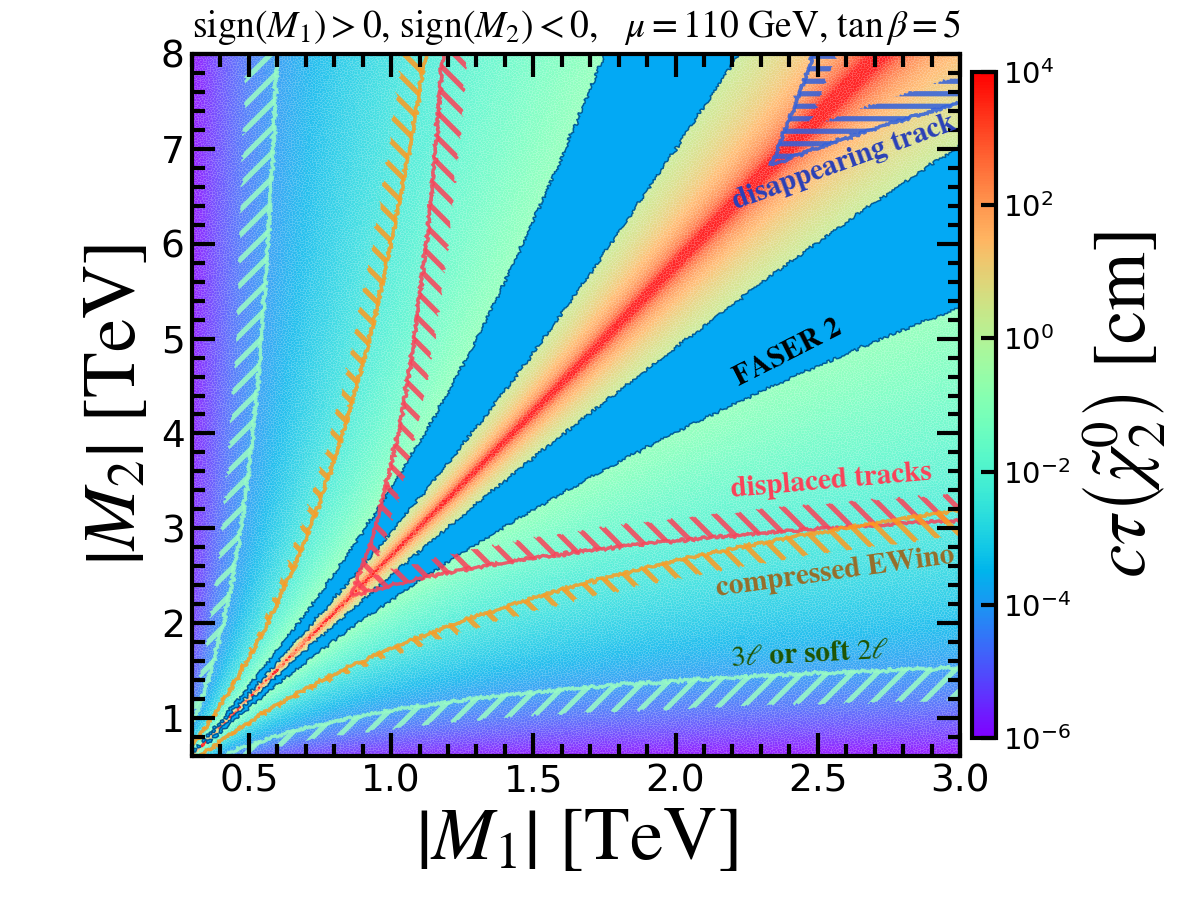
\includegraphics[width=0.495\linewidth]{mu110_TB05_M2minus.png}\\
    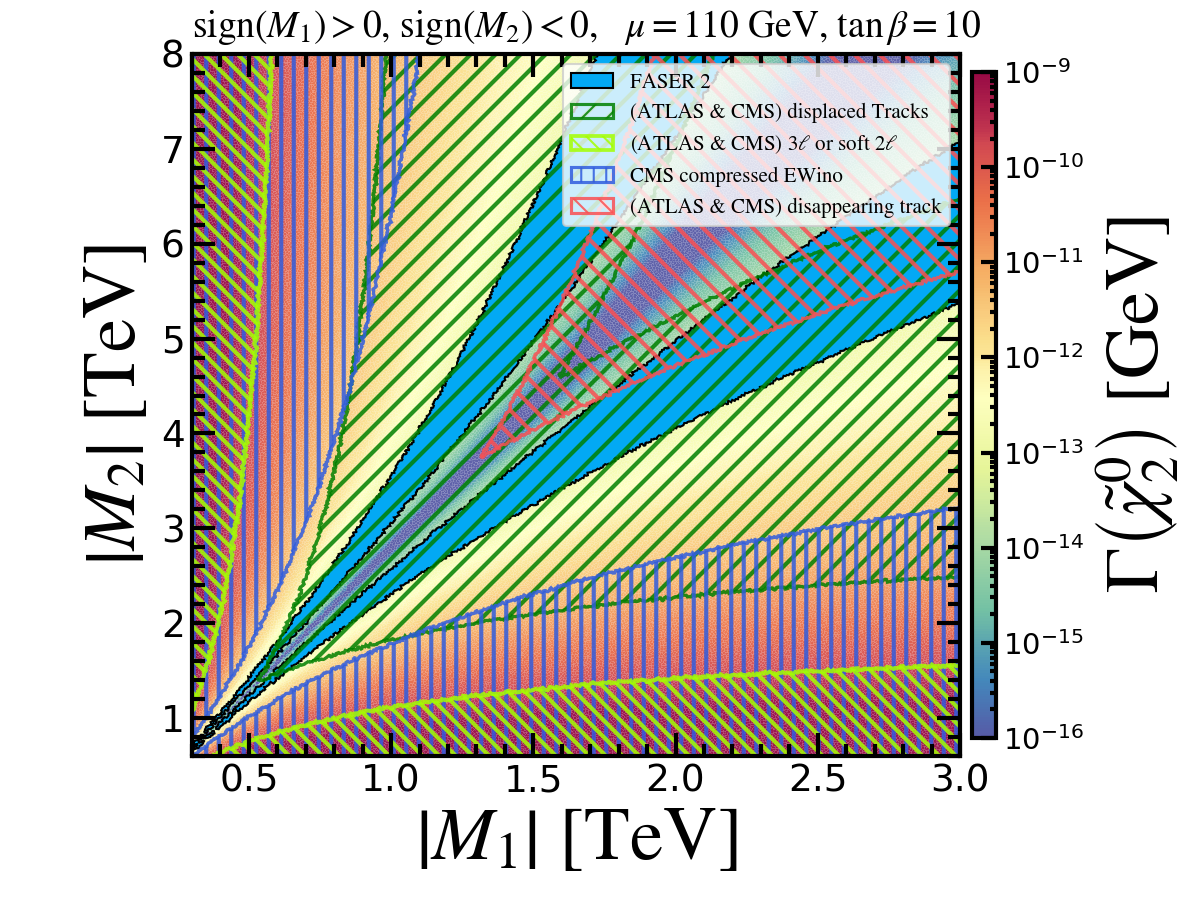
\includegraphics[width=0.495\linewidth]{mu110_TB10_M2minus.png}
    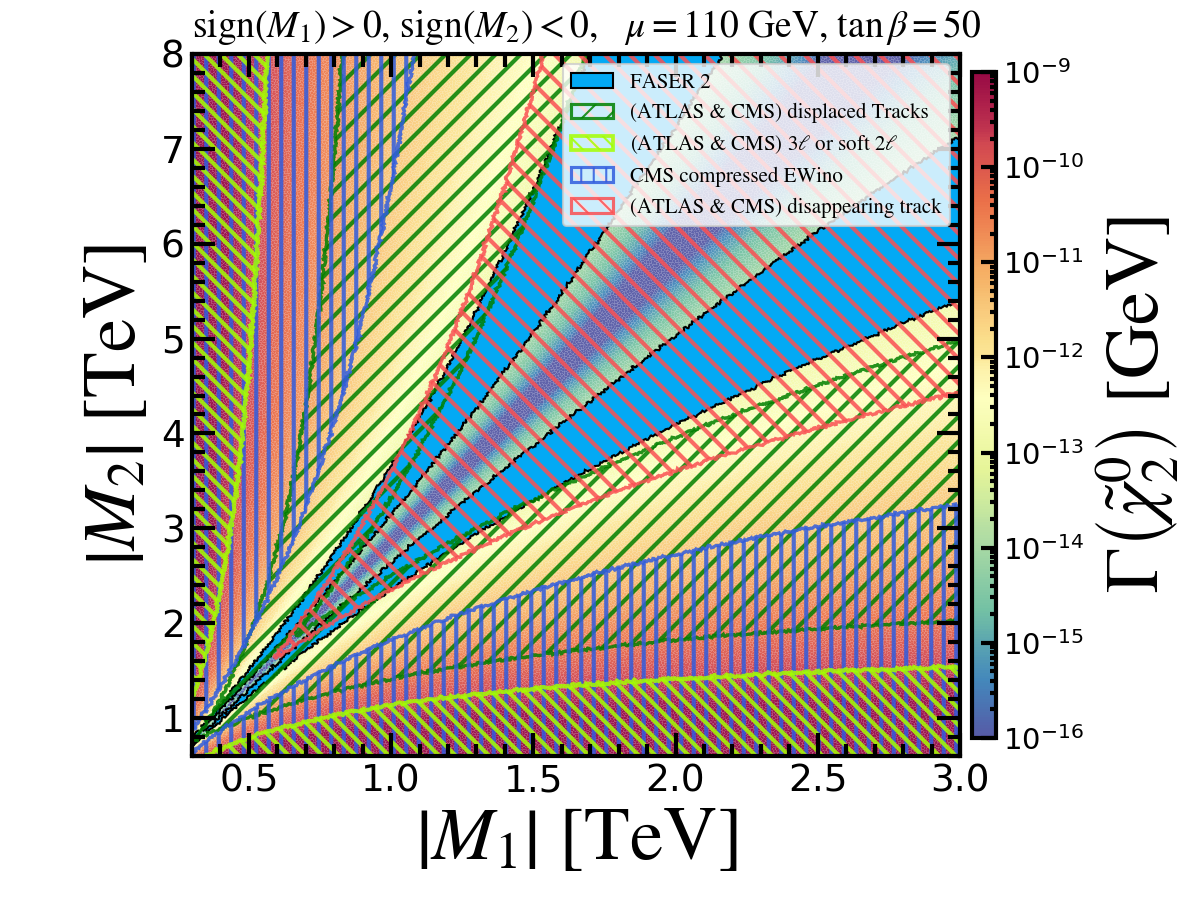
\includegraphics[width=0.495\linewidth]{mu110_TB50_M2minus.png}

    \vspace{-.3cm}
    \caption{\label{fig:ps} The coverage of the LHC searches and FASER 2 in the MSSM electroweakino parameter space is shown in the $(|M_1|,|M_2|)$ plane, with color shading representing the decay width $\Gamma(\tilde{\chi}_2^0)$. }
\end{figure}

\par The expected FASER 2 detection ability of the long-lived neutralino $\tilde{\chi}_2^0$ was shown in Fig.~\ref{fig:expconstrain}. FASER 2 increases sensitivity to regions where the mass difference $\Delta m^0$ ranges from $0.1$ to $0.5~{\rm GeV}$ for a higgsino mass of $100~{\rm GeV}$. The FASER 2 detection limit for the $\tilde{\chi}_2^0$ mass is approximately $126~{\rm GeV}$, with a corresponding mass splitting of 0.3 GeV. 
In conjunction with Fig.~\ref{fig:dkdm}, we observed that the value of $\tan{\beta}$ in EWMSSM parameter space has tiny impact on the decay of $\tilde{\chi}_2^0$. The detection ability for FASER 2 corresponding to $\tan{\beta}$ values of 2 and 50 differ slightly. 

The FASER 2 experiment provides a unique opportunity to explore the MSSM electroweakino parameter space, particularly focusing on the higgsino LSP with wrong-sign gauginos. In Fig.~\ref{fig:ps}, we present the current LHC search coverage and the projected sensitivity of FASER 2 for various $\tan{\beta}$ values in $|M_1|$ versus $|M_2|$ panels, with $\mu = 110~{\rm GeV}$. Conventional LHC searches, including those based on displaced tracks, soft-lepton signatures, and disappearing tracks, are illustrated with their respective exclusion regions. These analyses become less sensitive when the mass difference $\Delta m^0$ is small, while $\Delta m^\pm$ is significantly larger. For $\mu = 110~{\rm GeV}$, FASER 2 can detect the decay width of $\tilde{\chi}_2^0$ in the region of $8.8\times 10^{-15}~{\rm GeV}$ to $1.5\times 10^{-13}~{\rm GeV}$. This parameter space is shown as two bands in the $M_1-M_2$ plane, corresponding to the ratio of $M_2/M_1$ approximately within the interval $[-4.3, -3.4]$ and $[-2.3, -1.8]$. When $ M_2 $ is significantly large, the chargino becomes long-lived due to the small mass difference with the LSP $\tilde{\chi}_1^0$. In parameter space with a small $\tan{\beta}$ and ${\rm sign}(\mu M_2) < 0$, a large mass splitting between the chargino and the LSP is predicted. 

\begin{figure}[t]
\centering
    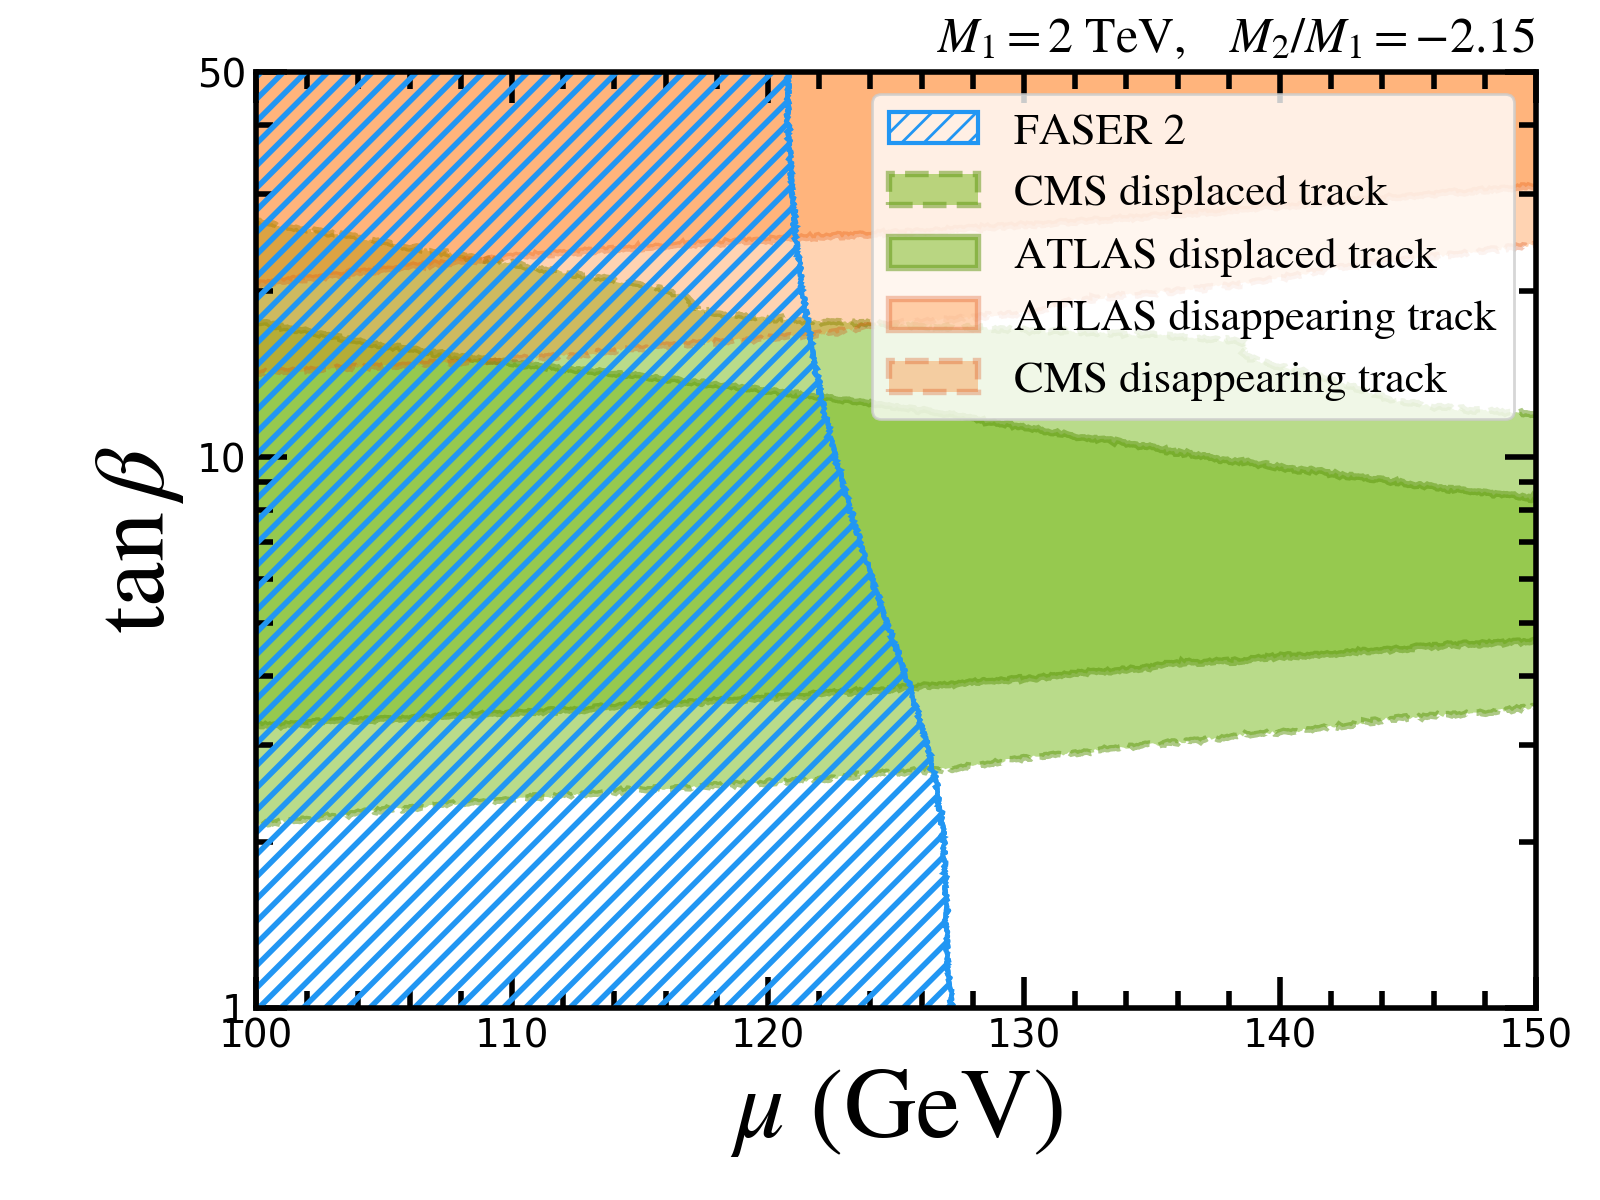
\includegraphics[width=0.495\linewidth]{muTB_logY.png}
    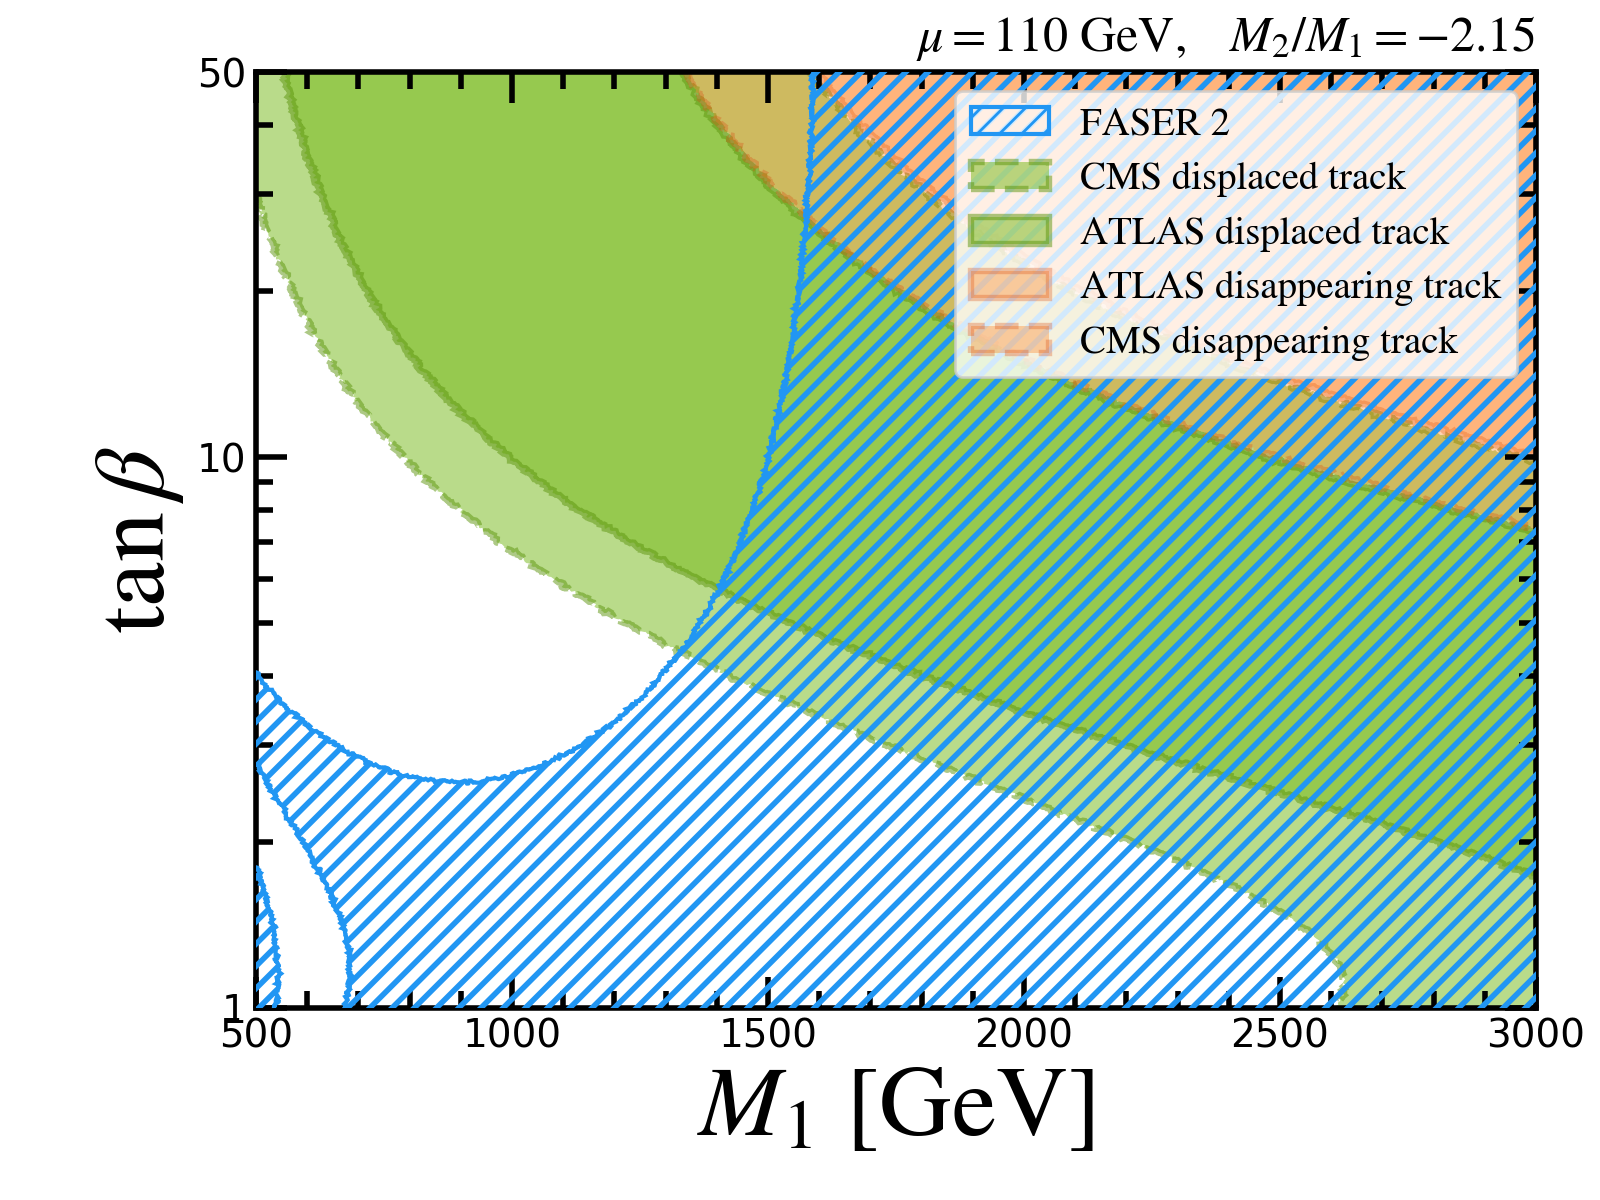
\includegraphics[width=0.495\linewidth]{M1TB_logY.png}
    \caption{\label{fig:ps2}Projected sensitivity of the LHC and FASER 2 in the $(\mu,\tan\beta)$ (left) plane and $(M_1, \tan\beta)$ (right) plane. \Shufang{log scale in tanbeta.}
}
\end{figure}
We then selected a specific $M_2/M_1$ ratio to examine the sensitivities of FASER~2 and current LHC searches to the MSSM parameter space. In Fig.~\ref{fig:ps2}, $M_2/M_1$ is set to $-2.15$. This configuration predicts that a long-lived Higgsino-like $\tilde{\chi}_2^0$ would exhibit high sensitivity in FASER~2, while remaining undetectable in standard LHC searches. In this case, only the LHC searches for long-lived chargino state $\tilde{\chi}_1^\pm$ can explore this specific parameter space. In the left panel of Fig.~\ref{fig:ps2}, with $M_1$ set to $2~{\rm TeV}$, nearly all regions where $\tan{\beta} \gtrsim 2$ are excluded by ATLAS/CMS searches for displaced or disappearing tracks. FASER~2 can be sensitive to the entire range of $\mu$ values below $123~{\rm GeV}$. In the right panel of Fig.~\ref{fig:ps2}, the mass splitting $\Delta m^\pm$ decreases as both $M_1$ and $\tan{\beta}$ increase. Consequently, LHC searches focus on the upper right regions. FASER~2 clearly complements the ATLAS/CMS searches shown in Fig.~\ref{fig:ps} and Fig.~\ref{fig:ps2}, underscoring the unique detection capabilities of FASER~2 for the MSSM parameter space.


\section{Conclusions}
\label{sec:sum}
Collider searches for higgsino-like LSP scenarios often rely on the general mass relation $m_{\tilde{\chi}_1^\pm} \approx |\mu| \approx ( m_{\tilde{\chi}_2^0} + m_{\tilde{\chi}_1^0})/2$. In this paper, we investigated a specific scenario within the MSSM electroweakino sector that breaks this relation, characterized by $\mu \sim 100~{\rm GeV}$, $|\mu| \ll |M_1|, |M_2|$, and a gaugino mass ratio $M_2/M_1 \approx -\tan^2{\theta_W}$. Under these conditions, the higgsino-like neutralinos $\tilde{\chi}_1^0$ and $\tilde{\chi}_2^0$ become nearly degenerate in mass, resulting in a long-lived $\tilde{\chi}_2^0$.

\par The region of parameter space with a small $\tan\beta$ and ${\rm sign}(\mu M_2) < 0$ is particularly challenging to probe with conventional LHC searches. However, the upcoming FASER2 experiment has the potential to explore this regime, with a sensitivity to a long-lived $\tilde{\chi}_2^0$ neutralino with mass around $126~{\rm GeV}$ and a mass splitting $m_{\tilde{\chi}_2^0} - m_{\tilde{\chi}_1^0} \sim 0.3~{\rm GeV}$. This corresponds to a decay width of $\Gamma(\tilde{\chi}_2^0) \sim 10^{-13}~{\rm GeV}$, highlighting the FASER 2 unique capability to probe scenarios inaccessible at traditional collider experiments.

\par The results in this paper are based on a straightforward and well-founded SUSY scenario. Unlike other models, where the long-lived particles are generated in rare decays of hadrons like $B$-mesons, in this scenario the long-lived $\tilde{\chi}_2^0$ is produced directly at the LHC interaction point via electroweak processes. Notably, our analysis showed that FASER~2 can significantly extend the sensitivity to long-lived particles with masses at the electroweak scale, greatly enhancing the experimental reach beyond current searches.

\addcontentsline{toc}{section}{Acknowledgments}
\acknowledgments
SS is supported by the Department of Energy under Grant No. DE-
FG02-13ER41976/DE-SC0009913. 
WS is supported by the Junior Foundation of Sun Yat-sen University and Shenzhen Science and Technology Program (Grant No. 202206193000001,
20220816094256002). 
JMY is supported by the National Natural Science Foundation of China under Grant No. 12335005 and by PI Research Fund from Henan Normal University under Grant No. 5101029470335. 
PZ is supported by the ARC Discovery Project DP220100007 and by the Centre for the Subatomic Structure of Matter (CSSM).
\appendix

\newpage
% \clearpage
\appendix
%\section{Supplemental Material}
\section{Introduction-short}
% \label{sec:intro}
Low-energy supersymmetry (SUSY) is one of the most compelling extensions of the Standard Model (SM) of particle physics, providing a natural solution to the hierarchy problem, enabling a unification of gauge couplings, and offering a viable dark matter (DM) candidate~\cite{Dreiner:2023yus, Martin:1997ns, Wang:2023suf, Haber:1984rc, Bae:2014yta}. However, the continuing searches at the Large Hadron Collider (LHC) are increasingly pushing up superpartner masses, raising the question of which superpartners are most likely to be detected at the LHC \Wei{refs}.

\par In this context, many studies have shown that the light higgsino scenario remains under-explored by the LHC, and the DM detection limits have not yet reached the exclusion threshold~\cite{Martin:2024ytt, Martin:2024pxx}. 
The higgsino mass parameter $\mu$ is unique in SUSY theory as it is the only SUSY-conserving term in the superpotential ($W \in \mu H_u H_d $).
In natural SUSY scenarios, the $\mu$ parameter is required to be close to the electroweak scale in order to avoid excessive fine-tuning in the electroweak symmetry breaking~\cite{Feng:2013pwa, vanBeekveld:2019tqp, Barbieri:1987fn, Arvanitaki:2013yja, Evans:2013jna, Baer:2014ica}. 
% Another possibility of light higgsinos arises in split SUSY where the electroweakinos, particularly the higgsinos, remain near the electroweak scale~\cite{Wells:2003tf, Arkani-Hamed:2004zhs, Wells:2004di, Arvanitaki:2012ps}. When the higgsino is the lightest SUSY particle (LSP), it can serves as a DM candidate, potentially providing the correct DM relic density with a mass of approximately $1.1~{\rm TeV}$~\cite{Delgado:2020url, Fox:2014moa, Chattopadhyay:2005mv, Chakraborti:2014fha, Shafi:2023sqa, Mummidi:2018myd}. Alternatively, if the higgsino mass is less than $1.1~{\rm TeV}$, other forms of DM are needed to account for the remaining density~\cite{Baer:2025srs}, or alternative non-thermal freeze-out sources must be considered~\cite{Han:2019vxi, Kowalska:2014hza, Aparicio:2016qqb, SuryanarayanaMummidi:2020ydm}. 
In the non-minimal SUSY models, light higgsinos could play a unique role in the thermal history of the early Universe~\cite{Cao:2018rix, Cao:2019qng, Cao:2019evo, Cao:2021lmj, Cao:2021tuh, Yue:2025dqe, Liang:2025utb, Dong:2024juh, Wang:2024ozr, Chakraborti:2024pdn, Dai:2023pli, Khan:2025yit}. Other intensive discussions about higgsinos are presented in recent works~\cite{Araz:2025bww, Zhou:2025xol, Carpenter:2023agq, Baer:2025zqt, Baer:2024hqm, Nagata:2025ycf, Baer:2024tfo, Fowlie:2024nhs, Li:2023hey, VanBeekveld:2021tgn, Baer:2020sgm, Bae:2019dgg, Baer:2017pba, Wang:2016otm, Fan:2024jvz, Du:2023qvj, Wang:2023bmh, Li:2022zap, Wang:2022rfd, Wang:2018idz, Khan:2025azf, Yin:2024bwv, Fu:2023sfk, Agin:2024yfs, Rodd:2024qsi, Liu:2020muv, Liu:2020ctf, Zhao:2022pnv}. 

Despite of the null results, current LHC searches still leave certain regions of the higgsino parameter space unexplored. The search for higgsino pair productions at the LHC faces several challenges. Due to the small mass differences 
$\Delta m^0 \equiv m_{\tilde{\chi}_2^0} - m_{\tilde{\chi}_1^0}$, 
$\Delta m^\pm \equiv m_{\tilde{\chi}_1^\pm} - m_{\tilde{\chi}_1^0}$, 
between higgsinos, the pair productions of $\tilde{\chi}_1^0 \tilde{\chi}_2^0$, $\tilde{\chi}_1^\pm \tilde{\chi}_2^0$ and $\tilde{\chi}_1^+ \tilde{\chi}_1^-$ lead to very soft visible decay products, as most of the energy is carried by the rest mass of the two LSPs. In most of the electroweakino parameter space with a higgsino LSP, the two mass splittings generally satisfy the relation $\Delta m^0 \sim 2 \Delta m^\pm$, which is widely used as a simplified model for LHC searches~\cite{LHCNewPhysicsWorkingGroup:2011mji, Canepa:2020ntc}. 
% 
It may imply that the true theory differs significantly from the simplified model. At same time, most of these studies show a uncovered window with very tiny $\Delta m^0$. This window, on one hand, is beyond the capability since the signals are not easy detected by the currently LHC. On the other hand, it shows some new features, which may be detected by other machines. Especially, we find that such a tiny $\Delta m^0$ could result to long-lived $\chi^0_2$, generating a totally different signal. To cover this kind of signal, we here focus on the Long-lived Particles (LLPs) detection ability of ForwArd Search ExpeRiment (FASER) \Wei{refs}.

\Wei{How about focusing on the $\mu$ and uncovered compressed spectrum }
\Wei{about Faser, we may focus on the special long-lived signal, which will be coved by Faser~2 partially, enhancing the detector ability beyond 5 GeV?}
% 
% As pointed out in Refs.~\cite{Baum:2023inl, Chakraborti:2024pdn}, the decay mode $\tilde{\chi}_2^0 \to \tilde{\chi}_1^0 \gamma$ remains challenging to detect at the current LHC~\cite{ATLAS:2024woy} and diminishes the strength of leptonic signals~\cite{Constantin:2025mex}. Recent studies~\cite{Martin:2024pxx, Martin:2024ytt} demonstrate how a realistic model parameterization affects higgsino mass splittings and related dark matter observations, breaking the simplified relation $\Delta m^0 \sim 2 \Delta m^\pm$. As a result, we will focus on this special case where the potential signals are of long-lived particle (LLP) out of reach of the current LHC. 
It is a currently operating experiment at the LHC that can detect long-lived particles produced in the forward region of the ATLAS interaction point (IP). Mostly the LLPs travel in the very forward region,  and decays in FASER (480 meters from the IP) into two very energetic particles~\cite{Feng:2017uoz,FASER:2018ceo, FASER:2018bac, FASER:2022hcn, FASER:2021ljd,FASER:2021cpr}. At the HL-LHC,  FASER will be upgraded to FASER 2 with a larger volume of the detector~\cite{FASER:2018eoc,Anchordoqui:2021ghd,Feng:2022inv}, to have a better performance. 
%Generally, the FASER and FASER 2 mainly focus on light particles, produced from massive mesons in the forward region......XXX....
%

\par To perform the process, we work on a class of SUSY models where sub-TeV sparticles are higgsino-like states. The model is characterized by electroweakino parameters satisfying $|\mu| < |M_1|, |M_2|$ and ${\rm sign}(M_1 M_2) < 0$, where the simplified relation $\Delta m^0 \sim 2 \Delta m^\pm$ is usually broken and a long-lived higgsino like $\tilde{\chi}_2^0$ state can not be probed by the ATLAS or CMS experiments. Such a scenario may be accessible at the FASER or Faser~2, which are designed to search for long-lived particles with small mass differences and minimal visible decay signatures. 

\par This paper is organized as follows. 
In Sec.~\ref{sec:model}, the electroweakino sector in MSSM is revisited, and the higgsino mass splittings $\Delta m^0$ and $\Delta m^\pm$ are discussed in detailed. 
Sec.~\ref{sec:exp} summarizes the current LHC searches for higgsinos and the related simplified models. 
In Sec.~\ref{sec:faser}, we provide a brief introduction to the FASER experiments and then calculate the sensitivity of the FASER 2 experiment to the long-lived higgsino-like $\tilde{\chi}_2^0$.  
Conclusions are drawn in Sec.~\ref{sec:sum}.



\bibliographystyle{JHEP}
\bibliography{ref_type1}



\end{document}
